%%*********************************************************************%%

\documentclass[10pt, conference, letterpaper]{IEEEtran}

\IEEEoverridecommandlockouts
%\usepackage{cite}
%\usepackage{makecell}

%\usepackage[cmex10]{amsmath}
\usepackage{color}
\usepackage{graphicx}
\usepackage{tabularx}
\usepackage{algorithm}
\usepackage{algorithmicx}
\usepackage[noend]{algpseudocode}
\usepackage{amssymb,amsmath}
\usepackage[tight,footnotesize]{subfigure}
\usepackage{flushend}
\usepackage{listings}
\usepackage{color}
\usepackage{verbatim}
\flushend


\newtheorem{definition}{Definition}
\newtheorem{proof}{Proof}
\newtheorem{theorem}{Theorem}
\newtheorem{lemma}{Lemma}
\newtheorem{example}{Example}
\newtheorem{remark}{Remark}

\DeclareMathOperator*{\argmax}{arg\,max}
\DeclareMathOperator*{\argmin}{arg\,min}

%to replace our system name here, a user-define marco
\newcommand{\sysname}{\textsc{STAMP}}
%\textcolor{red}{}

\begin{document}
%
% paper title
% can use linebreaks \\ within to get better formatting as desired
\title{A Virtual Middleboxes Placement Algorithm in Multi-tenant Datacenter Networks}

\author{\IEEEauthorblockN{Jian Wang, Xuewei Zhang, Xiaoliang Wang, Sanglu Lu}
\IEEEauthorblockA{National Key Laboratory for Novel Software Technology\\
Nanjing University, Nanjing, P.R. China\\
Email: waxili@nju.edu.cn}
\and
\IEEEauthorblockN{Layong Luo}
\IEEEauthorblockA{Microsoft Research\\
Email: laluo@microsoft.com}
\and
\IEEEauthorblockN{Camtu Nguyen}
\IEEEauthorblockA{Lextend Corp.\\
ncamtu@gmail.com}
}


% make the title area
\maketitle


\begin{abstract}
Hardware middleboxes are widely used in current cloud datacenter to provide network functions such as firewalls, intrusion detection system, load balancers, etc. Unfortunately, they are expensive and unable to offer customized functions for individual tenant. To overcome this issue, there is an increasing interest in deploying software middleboxes to enable flexible security, network access functionality. This paper addresses the software middleboxes placement problem with minimum bandwidth guarantee. We first specify the model of tenants' requirement that specifies the need for virtual machines of application and middleboxes, as well as communication traffic. A virtual middlebox placement algorithm called EMB (short for Exchanging MiddleBox and application) \begin{comment}STAMP(short for SofTwAre Middlebox Placement)\end{comment} 
is then proposed to offer predictable network performance for each accepted tenant, and minimize  datacenter bandwidth utilization. Extensive simulation results based on current large-scale datacenter networks verify that EMB can accept more tenant requests than existing placement algorithm(e.g., Stratos) while saving almost 10\% more high-level links' bandwidth.
%is effective and provides network performance guarantee for tenants. 
\end{abstract}

\IEEEpeerreviewmaketitle

\section{Introduction}
Large public clouds, such as Amazon EC2 and Windows Azure, provide infrastructure as a service (IaaS) for enterprises and individuals. Besides the ability to provide computing resources, public clouds are expected to support network functionality, such as load balancers, firewall, intrusion detection system, etc. Currently, network functions are widely deployed by the expensive hardware middleboxes (HW MBs). As illustrated in Fig. \ref{fig:topo}, hardware middleboxes are placed at the point close to the data center switches. Since hardware middleboxes are shared by all tenants, it is hard to manage these expensive devices to provide customized functions for each tenant. Also, heavy congestion may happen at links around those middleboxes. To address these issues, cloud providers and researchers introduce software middleboxes (or, interchangeably, virtual middleboxes, middlebox VMs) in the cloud \cite{G13dio, stratos12}. % As a result, enterprises can compose complex network functionality on general-purpose servers, and enhance the availability, security and scalability of their services. Recent advances in this direction show that software middleboxes running on commodity servers are capable of working at line speed \cite{D12tpp, S12dai, netvm}.


% A sort of properly selected parameters are given to specify not only the tenants' application and middlebox VMs requirements, but the corresponding intra- and inter-tenant communication pattern.
Providing virtual middleboxes with guaranteed performance is challenging for cloud service providers due to several reasons. First, we need to model various requirements of tenants, which consist of application VMs, middlebox VMs as well as the connecting network. Second, the performance of software MBs is not easy to predict in real environment due to many factors like the number of rules, algorithms and implementations. The experience based selection of MBs may under- or over-estimate resource consumption. Last but not least, it requires an algorithm to efficiently place virtual middleboxes in cloud service infrastructure.


Inspired by recent works on application-driven bandwidth guarantee \cite{B13cta, cloudmirror}, we consider the middlebox placement strategy to overcome these challenges. Tenant's requirements is represented by a weighted directed acyclic graph (DAG). The nodes consist of diverse virtual middleboxes and a set of homogeneous application VMs, both of which are dedicated for each tenant to process arrival traffic. The edge of DAG indicates the communication request of middlebox-to-middlebox, middlebox-to-application traffic and intra-applications. The weight on the edge is the minimum communication requirement between application VMs \cite{stratos12, B11tpd}. The inter-tenant communication \cite{B13cta} is also structured by a directed network. The arrival traffic from other tenants will be forwarded to the MBs of the target tenant before arriving at its application VMs.




Existing placement algorithm showed in Stratos \cite{stratos12} seeks to partition the VMs into per-rack partitions and tries to place them with minimal inter-partition communication. However, the communications among partitions may travel through several switches due to improper rack selections even the partitions can be placed under the same switch since the algorithm only considers the VM slots and bandwidth resources when selecting the racks to accomadate the partitions, which leads to a bandwidth waste of core-level links.  
In contrast, %based on the model of tenant request, 
we first traverse the datacenter topology in a bottom-up manner to search for a valid lowest level subtree for the tenant request, and then carefully places the required MBs and application in form of VMs under the subtree. 
%we design an effective algorithm that carefully places the required MBs and application in form of VMs in datacenter to maximize the utilization of resources (e.g., computation and network).
%Moreover, to address the bandwidth constraint in an oversubscribed datacenter networks, we adopt the depth-first search (DFS) allocation algorithm in the tree-like datacenter topology to minimize the network bandwidth occupancy for each accepted tenant. 
Moreover, to make good use of both physical machine resource and network bandwidth resource, we consider dividing the middleboxes and the application VMs proportionally and putting them in the same server or rack so as to occupy as many virtual machine slots as possible to eliminate unnecessary communication cross racks due to the unbalanced assignment of traffic processing capacity. Further, we try to colocate more application VMs to reduce the intra-tenant communication cost through carefully exchanging the positions of middleboxes and application VMs. If free slots or bandwidth is not enough, the middlebox chain and application VMs have to be placed separately but in closed sub-tree to reduce the bandwidth consumption caused by communication intra- and inter-tenants. 


\begin{figure}
	\centering
		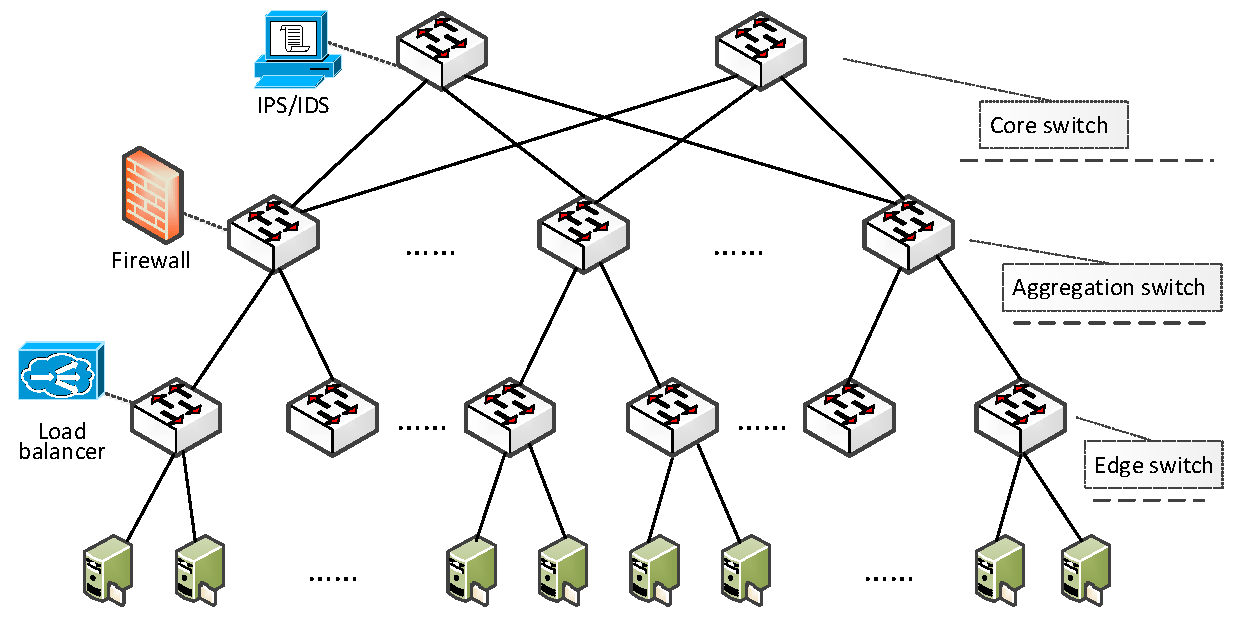
\includegraphics[width=3.2in]{fig/topology.pdf}
	\caption{Datacenter network and hardware middlebox deployment}
	\label{fig:topo}
\end{figure}

% Our virtual middleboxes network placement algorithm also takes into consideration some realistic constraints in the physical machine. For example, with SR-IOV \cite{sriov} enabled host visualization, the traffic of VM is directly forwarded (through DMA) to the network interface card. Therefore, the VM-to-VM communication inside a host is bounded by the maximum switching capacity in the network interface card (NIC). Due to the speed limitation on hardware switching inside NIC, it can not be improved by either increasing the number of virtual functions or cores \cite{netvm}. Thus we need to consider such reliability constraint during virtual MBs placement.


To the best of our knowledge, we are the first to model both the  virtual middlebox and application network placement problem in multi-tenant datacenter networks with minimal performance guarantees. Extensive simulations on large-scale datacenter topology have shown the effectiveness of our VMs placement algorithm. The accept ratio approaches to 90\% with regard to a variety of tenants' requests in a large-scale datacenter topology. Compared with the existing placement algorithm, our algorithm can also greatly reduce the bandwidth utilization of high level links while making the best of low-level links' bandwidth resource. %fragment that can not be used by newly arrived tenant requests. 
Compared with the hardware middlebox placements in current datacenters, our VMs placement shows significant saving on network bandwidth but provides the performance guarantee. Generally, the network function virtualization enables the cloud services provider to offer customized services with lower cost and our study will be helpful to build more flexible software-based cloud services to meet diverse requirements of  the tenants in the datacenter network.

%In general, we focus on tenant's requirement abstraction and effective VMs placement algorithm to achieve high network resource utilization in a datacenter. The contribution of this paper can be summarized as follows,
%\begin{itemize}
%	\item
%	\item the placement algorithm is effective and tested on our testbed.
%	\item moreover, we addressed the scalable issue of the mb placement which is the first time. because it is hard to evaluate the system requirement of mb, besides, the requirement is also variable.
%\end{itemize}

The rest of this paper is organized as follows. Sec. \ref{sec:background} reviews the background and related works on tenant's performance guarantee in the multi-tenant datacenter. Sec. \ref{sec:abstraction} describes our abstraction of middlebox and the communication model. The VMs placement algorithm is explained in Sec. \ref{sec:algorithm}, and the simulation based performance evaluation is demonstrated in Sec. \ref{sec:simulation}. Sec. \ref{sec:final} concludes this paper.

\section{Background and Related Works}\label{sec:background}
\textbf{Multi-tenant datacenter }
Large-scale datacenter is the core infrastructure for cloud based services. Datacenter network is organized in a multi-level tree-like topology. See Fig. \ref{fig:topo}, each rack typically contains 40+ servers, each of which is configured a 10Gbps network interface card (NIC) connecting to the top-of-the-rack (ToR) switch. The ToR switch will balance the traffic to multiple aggregation switches. All aggregation switches are further connected to the core switches. Note that the communication bandwidth between adjacent layers is oversubscribed by a ratio from 2:1 to 10:1, which may vary slightly with different configurations \cite{B13cta, williamson2010has}.

In multi-tenant data center environments, a tenant can rent multiple virtual machines (VMs) on physical servers. The VMs are configured with different amounts of CPUs, memories and storage resources. From the network perspective, we usually model the computation and storage resource to be the number of slots requested in physical machine. All VMs assigned to a tenant are interconnected to form a virtual network (VN) such that VMs can communicate with each other to exchange data. The traffic inside a multi-tenant datacenter carries external traffic to and from Internet, intra-tenant traffic between a tenant's application VMs and inter-tenant traffic. Specifically, the inter-tenant traffic consists of flows between tenants and flow between tenant and providers \cite{B13cta}, which can also be considered as a special tenant. Inter-tenant communication increases with the increase of services offered by cloud providers. Based on recent measurement in public cloud provider, 65\% of traffic happens between VMs belonging to one tenant VN and 35\% is among different VNs or tenant-provider communication \cite{B13cta, P13acs}.

\textbf{Middleboxes in multi-tenant datacenter }
Network functions are also necessary and provided in the form of hardware middleboxes in current datacenters.  However, hardware middelboxs are known to have several drawbacks. For example, working as a shared resource, the hardware middleboxes can only provide common services used by all tenants instead of providing customized tenant requests. Once the middlebox failed, all the tenants will be affected. Besides, the fixed locations of hardware middleboxes result in aggregated network bandwidth consumption and cause network congestion \cite{ClickOS, Y15NFV}. 

An alternative solution to hardware middleboxes is network function virtualization (NFV) \cite{NFV}. Deploying software middleboxes will greatly improve the flexibility, manageability and cost-efficiency. Software middlebox is not necessary to be shared and able to provide customized services with performance guarantee for each dedicated tenant. It has been shown that the software middleboxs are able to offer equivalent functionalists as the corresponding hardware implementation \cite{D12tpp, S12dai, G13dio, ClickOS}. The advance of software defined networking (SDN) further facilitates the deployment and management of software middlebox running in datacenters. Although there remains unsolved challenges before it can be integrated into the cloud ecosystem, the perspective of deploying flexible software middlebox for isolated tenants has motivated us to extend the previous works to realize predictable middlebox virtual networks through effective virtual middleboxes placement.


%SecondNet \cite{G10sad}, Seawall \cite{seawall}, Gatekeeper \cite{R11gsb}, Elastic Switch \cite{elasticswitch}, Oktopus \cite{B11tpd},
\textbf{Placement of services with performance guarantee}
Since the underlying network is shared by tenants, the application can be affected by variable and unpredictable network performance. A series of works have been proposed to enable traffic isolate and provide bandwidth guarantee, including Oktopus \cite{B11tpd}, FairCloud \cite{P12fst}, etc. The above works focus only on intra-tenant communication. The inter-tenant traffic isolation is addressed by Hadrian \cite{B13cta}. Through hierarchical hose model, the communication dependencies can be explicitly declared. The cloud provider then allocates resources according to the specification of tenants. 

Most of previous works only considered the bandwidth guarantee for applications. As far as we know, little work addresses the bandwidth guarantee for virtual MBs in multi-tenant datacenters \cite{7243304}. The NFV cloud computing platforms, like NFV OPEN LAB \cite{HuaweiNFV} and CloudNFV \cite{CloudNFV}, provide NFV management and orchestration as applications. Theoretically, to obtain effect use of resources, various NFV placement objectives have been studied, for example, remaining data rate, latency, number of used network node as well as distance and setup cost, see \cite{M14sap, cohen2015near} and the references therein. However, they could not provide bandwidth guarantee for tenants. Stratos \cite{stratos12} considered the middlebox placement in multi-tenant datacenters through a systematic way by avoiding network congestion. In contrast, we first study the bandwidth guarantee
%consumption
 problem of both virtual middleboxes and application and then propose effective placement algorithm to make good use of network resources.

\section{Abstraction of Virtual Middlebox Network}\label{sec:abstraction}
In a multi-tenant datacenter, by leveraging the network function virtualization (NFV), cloud providers provide middlebox as a fundamental network service to tenants, like both computing and storage resources. A tenant could specify their middlebox and application (i.e., computation/storage) requirements in forms of VMs and the expected minimum bandwidth requirement for intra- and inter-tenant communication. Cloud providers will then assign VMs for middleboxes (in short, MB VMs) and applications (in short, APP VMs) according to the tenant's request. The cloud providers also enforce the middlebox policies, i.e., the sequence of middleboxes that a flow must traverse. In this section, we explain the model for APP VMs and MB VMs. We then introduce the abstraction of virtual networks associated to one tenant.


\subsection{Model of APP VMs}
To provide predictable network performance for the communication of $N$ APP VMs in one tenant, users typically specify the minimum bisection bandwidth $B^{in}$ for individual APP VM. Analogous to previous proposals \cite{B13cta, P12fst}, the requirement of the minimum bandwidth guarantee for each APP VM belonging to the same tenant can be abstracted by the \emph{hose model}. In the hose model (see the thick black arrows in Fig. \ref{fig:hose}, tenant P), the application VMs are connected to a logical switch by a link of capability $B^{in}$.

\begin{figure}
	\centering
		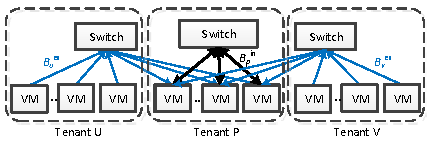
\includegraphics[width=3.5 in]{fig/tagmodel.pdf}
	\caption{Intra-tenant communication and inter-tenant communication}
	\label{fig:hose}
\end{figure}

Similarly, for the cross tenants communication, a tenant can specify the bandwidth request for a single APP VM. The minimum bandwidth guarantee for inter-tenant traffic of each APP VM is defined by $B^{ex}$. We extend the VN model of Hadrian \cite{B13cta} to support multiple external links. If the current tenant communicates to multiple tenants. The minimum bandwidth for each communication pair is guaranteed to be $B^{ex}$. The communication pattern between tenants can be expressed by a directed graph. We use the definition of \emph{communication dependency} in \cite{B13cta} to explicitly specify the peer-to-peer traffic pattern. A tenant with a dependency of \{*\} means that he could allow any other tenants' communication request. We call this kind of tenant open tenant while the tenant who has communication requests to open tenants are called client tenant. When the dependency is set as P:\{U, V\}, it means that the communication from tenant U and tenant V to tenant P are allowed. An example is illustrated in Fig. \ref{fig:hose}, the thin blue arrows show the communication between tenant U and tenant P, as well as tenant V and tenant P.

% Here is an example: i) A:\{B,C\}, ii) B:\{A\}, iii) C:\{*\}, which means that the communications between tenant A and tenant B, tenant A and tenant C are allowed. Therefore, the APP VMs' request of a tenant can be characterized by a four-tuple $<N, B^{in}, B^{ex}, dependencies>$.



\subsection{Model of MB VMs}\label{sec:modelformb}

Middleboxes perform different network functions to meet traffic demand of applications. A tenant may vary network functions simultaneously to process packets of different traffic class, as shown in Fig. \ref{fig:chain}. Each request consists of a sequence of various MBs, such as firewall (FW), intrusion detection system (IDS), redundancy elimination(RE), load balancer (LB) and NAT Proxy, etc., which provide functionality of access control and traffic engineering. 
% Notice that the software MBs are dedicated for each tenant. Due to the security and reliability, the assigned MBs will not be shared with other tenants based on the SLA requirement.  


Generally, the communication between MBs can be abstracted by a directed-acyclic graph (DAG), where the vertex represents the type of middleboxes and the arc indicates the traffic flow between them. The external traffic should pass through the specified middleboxes one by one according to the DAG. The sequence can not be violated. Otherwise, the expected functionality will be ruined. In addition, we assume that the traffic still keeps the same when multiple MBs are introduced. This is reasonable because the traffic is the minimum bandwidth guaranteed for both intra- and inter-tenant communication. The normal traffic could pass all the rule checking and will not be blocked by middbleboxes like FW or IDS. For those middelboxes, e.g., RE or LB, which change the traffic load, they are usually placed at the end of the DAG. The variation of traffic is specified by the proposed parameters of $B^{in}$ and $B^{ex}$ in the aforementioned APP VMs model.

\begin{figure}
	\centering
		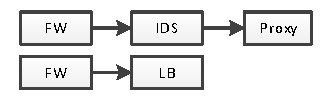
\includegraphics[width=3.0 in]{fig/chain.pdf}
	\caption{Abstraction of MBs: Two MBs chains}
	\label{fig:chain}
\end{figure}

% (important) However the abstraction of DAG may increase the representation and placement burden of middleboxes. Alternatively, the DAG can be simplified by partitioning the shared middleboxes to form multiple chains \cite{stratos12}. derived from the DAG given in Fig. \ref{fig:chain} (a) This operation is reasonable because a tenant can enable flow distribution at the head of DAG graph. , which classify the traffic 

Since a tenant may need to apply different middlebox policies to different traffic class, the tenant request can be classified into multiple MBs chains associated with different applications \cite{stratos12, M14sap, 7243304}. See Fig. \ref{fig:chain} as an example. The Internet traffic will pass Firewall, Intrusion Detection System and then NAT proxy, while the traffic from other tenant may only pass Firewall and Load Balancer. Therefore, a middlebox chain model can be defined by a tuple $\langle T, M \rangle$, where the type of MBs is denoted by a vector $T$, and the number of required MB VMs is denoted by a vector $M$. The direction of traffic flow is implicitly expressed by the sequence of items in the vector $T$. For instance, the first MB chain in Fig. \ref{fig:chain} can be expressed as $\langle T, M \rangle$, where $T=\{\text{FW, IDS, Proxy}\}, M=\{2, 4, 2\}$. It means that the tenant request for 2, 4 and 2 VMs of FW, IDS, and Proxy respectively. The traffic will arrive at FW first, and then go to IDS and pass Proxy before reaching the application VMs.

\subsection{Virtual Network Model for MB VMs and APP VMs} 
We combine the MB model and APP model together to form the virtual network (VN) model to represent the tenant's request. The interaction between VMs of the same tenant is expressed by the hose model. The middlebox chain should be attached to the ingress path of the external link of the VN. Such that, all external traffic coming into APP VMs must traverse through these specified middlebox chains which provide access control and other network functions. CloudMirror \cite{cloudmirror} provided a new network abstraction that allows the applications to specify their directional and specific communication pattern. We adopt a cascade of \emph{Tenant Application Graph (TAG)} proposed in \cite{cloudmirror} to specify the VN model. 

Fig. \ref{fig:abstraction} (a) shows an example, where a sequence of MBs is attached at the external link of APP VMs of tenants. The arrow shows the traffic flow. Arrival traffic of tenant A will pass through all these middleboxes before being distributed to the application services. Similarly,  the departure traffic of tenant A is forwarded to its destination (tenant P) which needs to pass through the middleboxes of tenant P first \footnote{Some corporations may have the requirement to detect the departure traffic through additional middleboxes. We leave this for future work. }.  Fig. \ref{fig:abstraction} (b) uses the cascade of TAG model to abstract the communication dependency of VNs. The external traffic passing through each type of middleboxes in sequence are expressed by the dedicated directional arrows. The internal traffic of APP VMs is expressed by bi-directional arrows, each of which has a capacity of $B_{A}^{in}$ (tenant A) or $B_{P}^{in}$ (tenant P). The external traffic of each VM of tenant A (resp. tenant P) is bounded by $B_{A}^{ex}$ (resp. $B_{P}^{ex}$). 
\begin{figure}
	\centering
		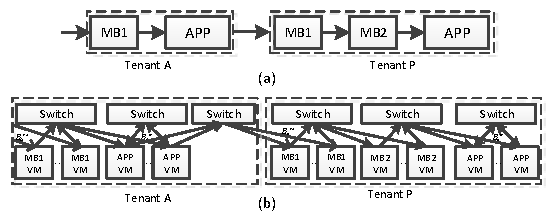
\includegraphics[width=3.5 in]{fig/abstraction.pdf}
	\caption{Virtual Network Model. (a) the communication between two tenants; (b) cascade of TAG}
	\label{fig:abstraction}
\end{figure}

% and 3) the traffic from the other VN belonging to the same tenant
In general, two kinds of traffic may go through the MBs before come to the Application VMs, 1) the Internet traffic; 2) the traffic from other tenant. When declaring a connectivity relationship, this external link can only communicate with those specified VNs. The unauthorized traffic will be blocked by MBs. Based on the models of APP VMs and MB VMs, a tenant can specify the connectivity of an external link which receives (or sends) traffic from any VN. In summary, a tenant's request can be specified by multiple virtual networks (VNs) and each VN can be specified by a tuple $<N, B^{in}, B^{ex}, dependencies, T, M>$. 

\noindent \textbf{Remark } 
It is a remarkable fact that the behavior of current software middleboxes is actually not easy to predict in the real system. The performance depends on multiple factors, including workload like traffic demands, type and number of rules, and middelbox design, e.g., algorithm design, systematical implementation, etc. Therefore, the scalability of MBs is important and need to be considered by the cloud service provider. Once the virtual network are placed in datacenter, it is hard to find a proper resource to migrate MBs and re-allocate live flows across MBs with performance guarantee \cite{G13dio}. We discuss the scalability issue in Appendix.

% Specifically, the VMs inside the blue dotted line are pre-allocated VMs for middleboxes subrequirement, which are shared by both types of middleboxes requests. If there are scale-out or failover request, specified MBs will be placed on these VMs to provide performance guarantee. 

\section{Virtual Middlbox Network(VMN) Deployment}\label{sec:algorithm}
Based on the tenant's request, the cloud provider allocates enough resources for MBs and APPs. The VMs request will be satisfied by providing enough free slots on physical machines (PMs). The network function demand consists not only the bandwidth request but also the capability to process a specific class of traffic in order. We present a VM placement algorithm that bridges the gap between the high-level virtual middlbebox network model to the low-level physical network. The placement strategy is realized by a logically centralized controller, which manages datacenter operations through a global view of the network topology. SDN based traffic engineering manipulates the underlying network routers to explicitly direct the class of traffic through each middlebox sequentially. If there are not sufficient resources, the request will be rejected. 


The virtual machine placement problems have attracted a lot of attentions recently, which are often formalized as a multi-dimensional packing problem with various constraints. This problem is NP-hard \cite{packing, fischer2013virtual}. %In this paper, 
Therefore, we search for effective heuristic solution to maximize the datacenter resources utilization. %Before introducing the VMs placement algorithm, we first explain some practical constraints in our design. Next, 
In this section, we first analyze the bandwidth requirement for the tenant request. Next, we give two placement principles according to the bandwidth requirement analysis. Finally, we present our placement algorithm to efficiently deploy the VMN model. 
%our placement stratety we present our placement strategy by combining two simple placement algorithms. 

%\begin{figure}
%	\centering
%		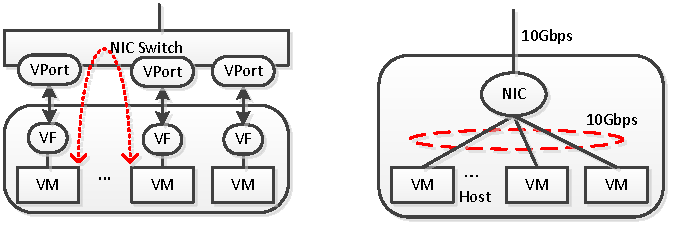
\includegraphics[width=3.5 in]{fig/nic.pdf}
%	\caption{Bandwidth constraint of NIC in PM}
%	\label{fig:nic}
%\end{figure}

%\subsection{Bandwidth Constraint within a Physical Machine}

%Existing operating systems typically copy the data from user space to kernel space and then move the data to the buffer of NIC. The data copies cause a long delay during packet transmission. Recent works allows applications to access the NIC card directly without involving kernel processing which direct DMA to and from a VM, like Single Root I/O Virtualization (SR-IOV) \cite{sriov}. Intel SR-IOV allows multiple VMs to access the NIC through L2 address. Most data center networks have enable the SR-IOV in their system to accelerate the data processing\footnote{Virtual Ethernet Port Aggregator (VEPA) forwards packets out of the host and come back via an external switch to be transmitted to a VM. Since VEPA will cost more network resource, we do not consider this situation in this paper.}. When using SR-IOV, packets are switched on a per-port basis in the NIC between VMs on a shared port, as that shown in Fig. \ref{fig:nic}. The hypervisor configures the NIC switch on the SR-IOV network adaptor to provide network connectivity to the VMs. However, the communication between VMs is bounded by the NIC switch capacity. NetVM \cite{netvm} tried to overcome this limitation by providing  memory sharing without passing through the NIC. However, due to some problems like the potential security thread in multi-tenant datacenter, this new feature is not applied in current commodity environment yet. In general, the bandwidth constraint inside PM can be expressed that the traffic between VMs of the same PM is bounded by a maximum bandwidth, see the model at right side of Fig. \ref{fig:nic}. We need to take this constraint into consideration during VMs placement algorithm design.

\subsection{Bandwidth Required by VMN}
%Giving a virtual network request, we need to provide enough middleboxes to process the traffic from the external Internet or other tenants. We assume each instance of $MB_k$ has a maximal traffic processing capacity $c_k$, So the minimum required number of $MB_k$ is:
%\begin{equation}
% M_{k}={\left\lceil\frac{N*B^{ex}}{c_{k}}\right\rceil}. 
%\end{equation}
%Then we can obtain the total number of VMs required for the middleboxes and applications. 
Given a tenant request, the cloud provider need to allocate sufficient bandwidth on the physical links to meet the bandwidth guarantees requirement specified in the VMN model.
For each VMN model, we assume that the total incoming traffic is shared equally among each instance of $MB_k$. And the practical required bandwidth $b_k$ for each instance of the same type MB can be calculated by :
\begin{equation}
\label{equ:bk}
b_{k}=\frac{N\cdot B^{ex}}{M_{k}}.
\end{equation}


\begin{figure}
	\centering
	     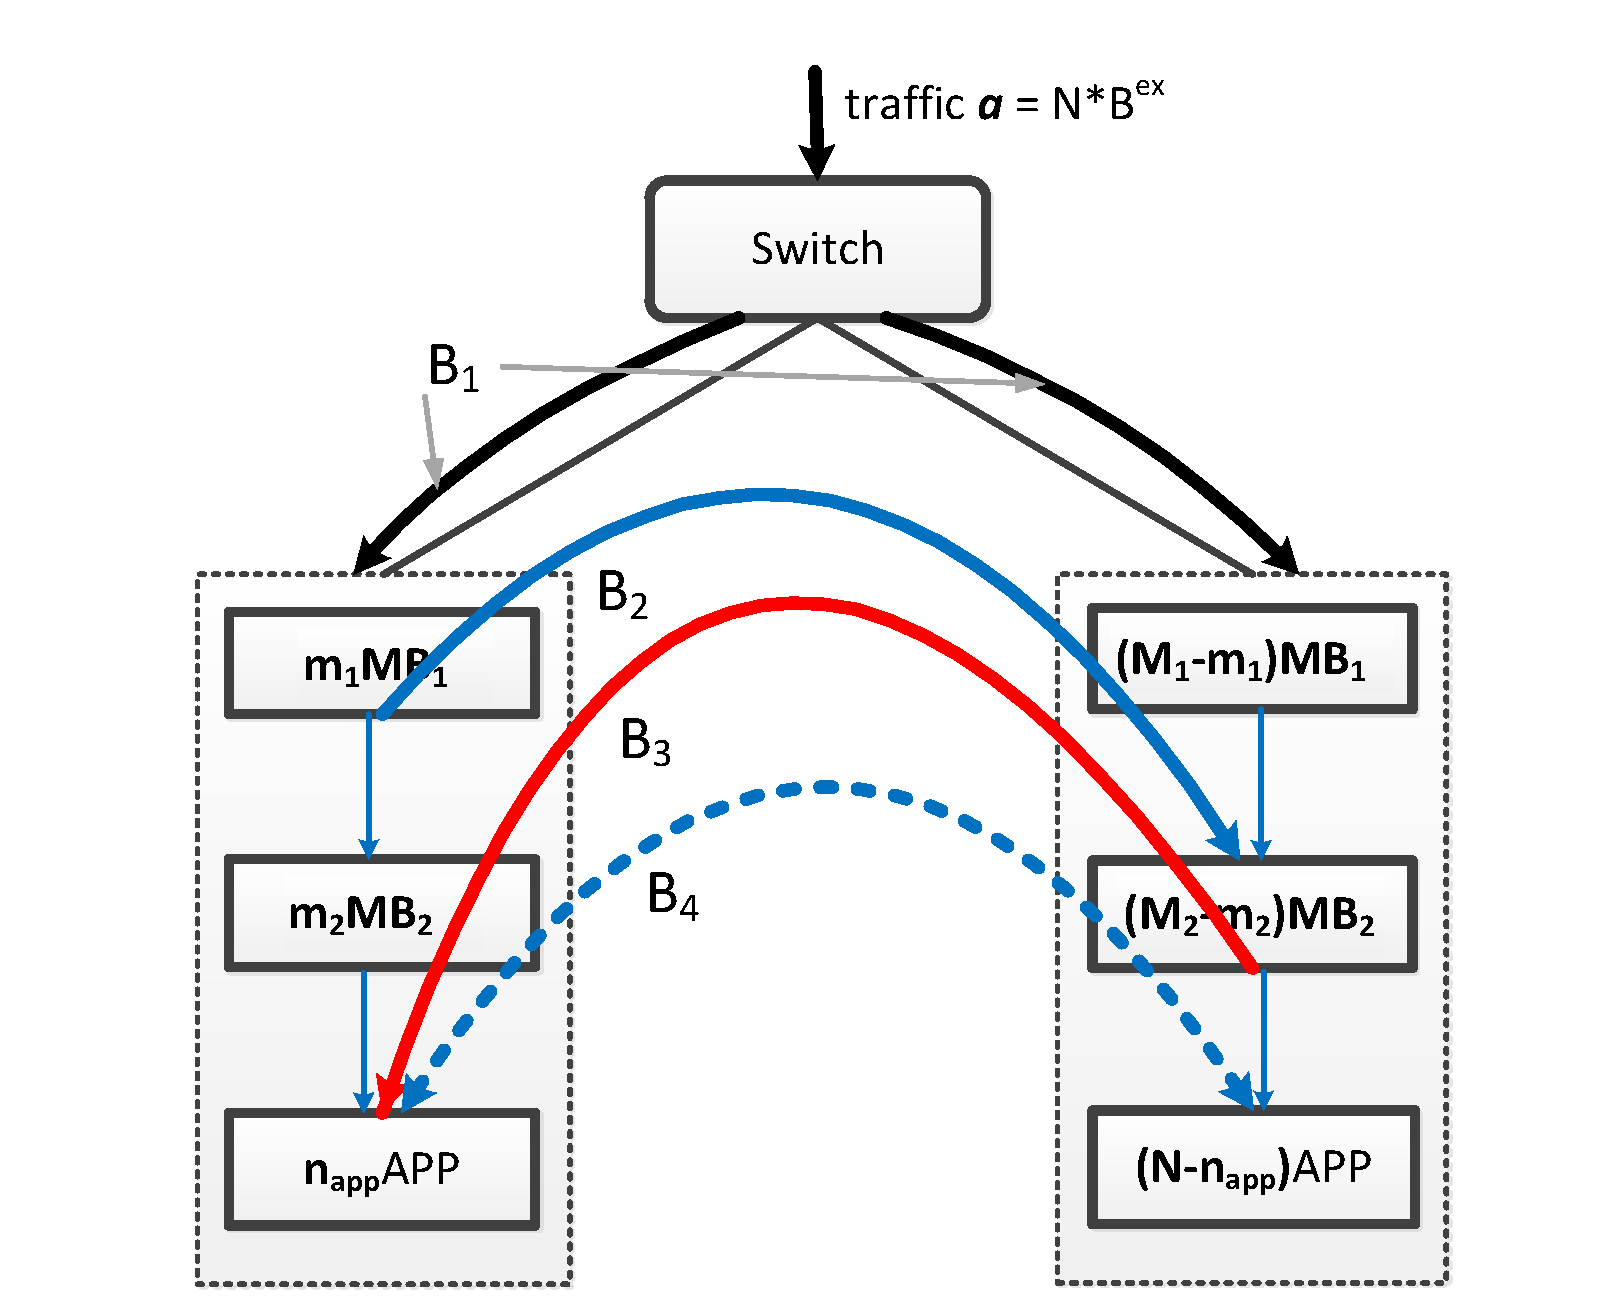
\includegraphics[width=3.2 in, height=2.5in]{fig/bandwidth_requirement.pdf}
	\caption{Bandwidth requirement}
	\label{fig:bw}
\end{figure}

\begin{comment}\begin{figure}
	\centering
	\subfigure[TRAIN: dividing virtual middleboxes network horizontally]{
		\label{fig:train} %% label for 2 subfigure
		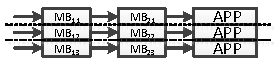
\includegraphics[width=3.0 in]{fig/train.pdf}}
	\subfigure[TRUCK: dividing virtual middleboxes network vertically.]{
		\label{fig:truck}%% label for 1 subfigure
		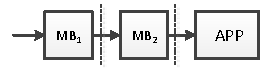
\includegraphics[width=3.0 in]{fig/truck.pdf}}
	\caption{Two partition strategies to distribute the VMs among subtrees}
\end{figure}

\begin{figure}
	\centering
	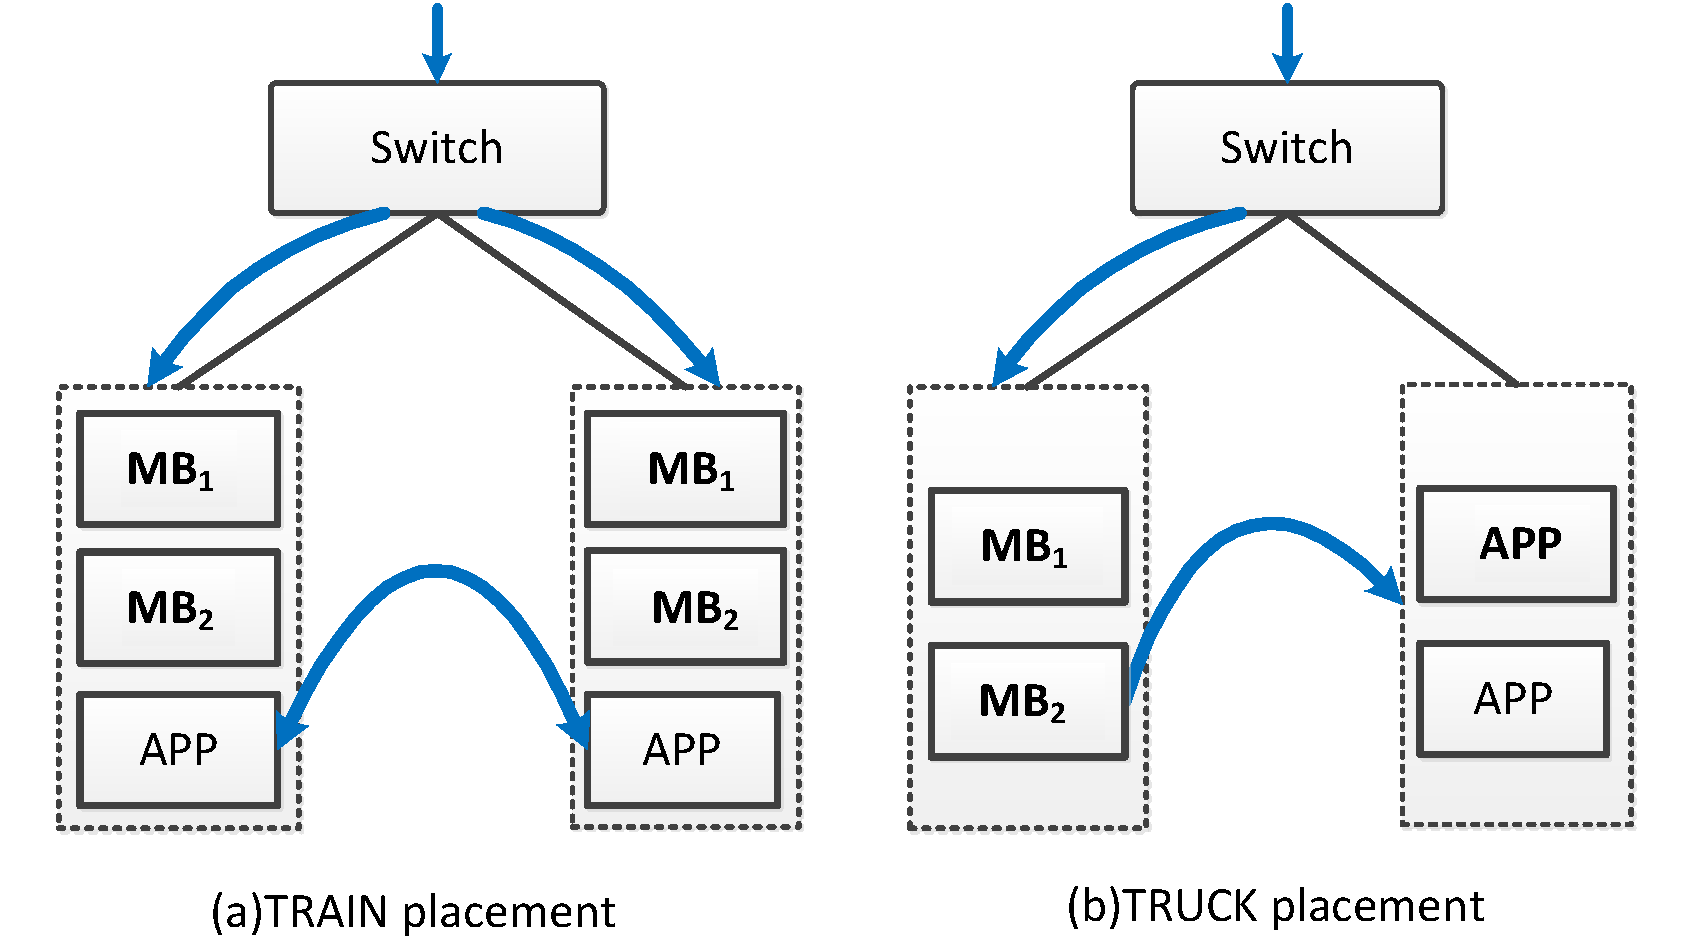
\includegraphics[width=3.5 in]{fig/train_truck.pdf}
	\caption{Illustration of placement algorithms}
	\label{fig:intuition}
\end{figure} 
\end{comment}
%\begin{figure}
%	\subfigure[]{}
%	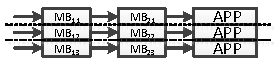
\includegraphics[width=3.5in]{fig/train.pdf}
%	\label{TRAIN:}
%\end{figure}
%In the subsequence,%
Based on above calculation, we analyze the bandwidth consumption to achive a better understanding of the MBs placement problem. Assume that we have found two candidate subtrees that have enough slots to hold the required VMs as shown in Fig. \ref{fig:bw}. The total number of instances required for $MB_k$ is indicated by $M_k$. And $m_k$ is the number of instances placed for $MB_k$  in the left subtree. %The number of VMs for the application is $n_{app}$ in the left subtree.%
 Correspondingly, the number of instances for $MB_k$ in the right subtree is $M_k-m_k$. The $n_{app}$ and $N-n_{app}$ are the number of APP VMs in the left and right subtrees respectively. Suppose the arrival traffic is $N*B^{ex}$ and the middlebox instances prefer to send the traffic to its downstream middlebox instances inside the same subtree.

We then calculate the bandwidth consumption. The traffic flows across and inside the subtrees are illustrated in thick and fine arrows respectively. Specifically, we find that the bandwidth consumption across the subtrees consists of four parts indicated by $B_1$, $B_2$, $B_3$ and $B_4$. The $B_1$ is the external traffic (represented by the black arrows) from the switch to $MB_1$ which is equal to $N\cdot B^{ex}$. The traffic that cannot be fully processed by $MB_2$ will be partly sent to the instances of $MB_2$ in the opposite subtree as shown in the blue arrow labeled by $B_2$. Similarly, the traffic from $MB_2$ in the right to APP will be partly sent to the APP VMs in the left subtree (red arrow labled by $B_3$) if the capacity of APP VMs in the right cannot serve the whole traffic from $MB_2$ in the same side. Besides, the bandwidth requirement (dotted arrow labeled by $B_4$) for intra-tenant communication is $2min⁡(n_{app}  ,N-n_{app})\cdot B^{in}$. For simplicity, we only consider the downlink bandwidth consumption since the uplink bandwidth has the similar characteristics. Based on above analysis, we can easily get the total downlink bandwidth requirement across the subtrees:
\begin{equation}
\begin{aligned}
bw = &B_1+B_2+B_3+B_4 \\
=&N \cdot B^{ex}+(m_1 \cdot b_1-m_2\cdot b_2)\\
&+((M_2-m_2)\cdot b_2-(N-n_{app})\cdot B^{ex})\\
&+2min(n_{app}, N-n_{app})\cdot B^{in}.
\end{aligned}
\end{equation}

For the general situation (i.e., the MBs and application VMs are randomly placed in the two subtrees), by adding all the inter-middlebox traffic going across the subtrees, we can get the following new equation:
\begin{equation}
\begin{aligned}
bw= &B_{switch,mb_{1}}+B_{mb_k,mb_{k+1}}+B_{mb,app}+B_{app}\\
 =&N\cdot B^{ex}+\sum\limits_{k=1}^{n-1}|m_k\cdot b_k-m_{k+1}\cdot b_{k+1}|\\
&+|m_n\cdot b_n-n_{app}\cdot B^{ex}|
\\&+2min(n_{app}, N-n_{app})\cdot B^{in}.
\end{aligned}
\label{equ:bw_equation}
\end{equation}
%For the general situation, by adding all the inter-middlebox traffic going across the subtrees, we can get the following (new) equation:
%
$B_{switch,mb_1}$ is the incoming traffic for $MB_1$ from the switch which is a constant. $B_{mb_k,mb_{k+1}}$ and $B_{mb,app}$ are the incoming traffic for $MB_{k+1}$ and APP VMs across the subtrees from $MB_k$ respectively. $B_{app}$ represents the intra-tenant communication bandwidth requirement.

%\subsection{Bandwidth Saving Conditions}
\subsection{VM Placement Strategy}
%Based on above bandwidth calculation, we can find two simple strategies to distribute the VMs among the subtrees. One approach is to always place all kinds of MB VMs in the same subtree proportionally with corresponding APP VMs. Each partition contains sufficient MBs to serve the APPs which can works independently. We call such approach 'TRAIN', since it works like a train consisting of multiple cars of MBs. As shown in Fig. \ref{fig:train}, it consists of three groups horizontally, each of which can process all arrival traffic to the APP VMs in the same group. Another approach is to make the same kind of MBs as a group and place them together in the subtree. We call this approach 'TRUCK' since it works like a truck to take cargo of the same kind. As shown in Fig. \ref{fig:truck}, $MB_1$, $MB_2$ and APP are divided first and put to subtrees separately.

%Fig. \ref{fig:intuition} shows the placement examples for above two simple strategies. The bandwidth comsumption across the subtrees is represented by the blue arrows. Obviously, the placement strategy TRAIN can minimize the bandwidth requirement from $MB_k$ to $MB_{k+1}$ and APP, but it may have a large bandwidth demand for intra-tenant communication. In constrast, TRUCK can save intra-tenant bandwidth greatly but having a big waste of bandwidth from $MB_k$ to $MB_{k+1}$ or APP. 


%Considering the advantages of the two strategies, we seek to obtain a more powerful placement algorithm to achive bandwidth saving by combining them. 
%\begin{comment}
We then obtain key conditions to achive bandwidth saving through careful placement of MB and APP VMs from Eq.\ref{equ:bw_equation}. We only consider the bandwidth requirement $B_{mb_k,mb_{k+1}}$, $B_{mb,app}$, and $B_{app}$ since $B_{switch,mb_1}$ is a constant. 
%\end{comment}
%Based on above results, 
More specifically, to reduce the traffic $B_{mb_k,mb_{k+1}}$ and $B_{mb,app}$ crossing the subtrees caused by the unbalanced capacity between the upstream and downstream MBs or APPs, we can place the MBs and APPs proportionally in the two subtrees according to their traffic processing capacity. In addition, as $n_{app}$ increases from zero to $N$, the intra-tenant bandwidth $B_{app}$ increases from zero to $2\cdot (N/2)\cdot B^{in}$ when $n_{app} = N/2$ and then derease to zero. So through colocating more APP VMs in one subtree, we can greatly save the intra-tenant bandwidth $B_{app}$ . 

%Thus, we get the following two placement principles:
Thus, we get the following two-step placement strategy: 1) placing the MBs and APPs proportionally according to their capacity initially and then 2) colocating as many APPs as possible through exchanging the positions of MBs and APPs in the two subtrees. While the exchanging may result in a change of bandwidth consumption due to the break of balance of MBs’ and APPs’ capacity. So we need to carefully select the MBs to exchange. We then analyze the change of the bandwidth before and after the exchange of the MB and APP.

\begin{figure}
	\centering
	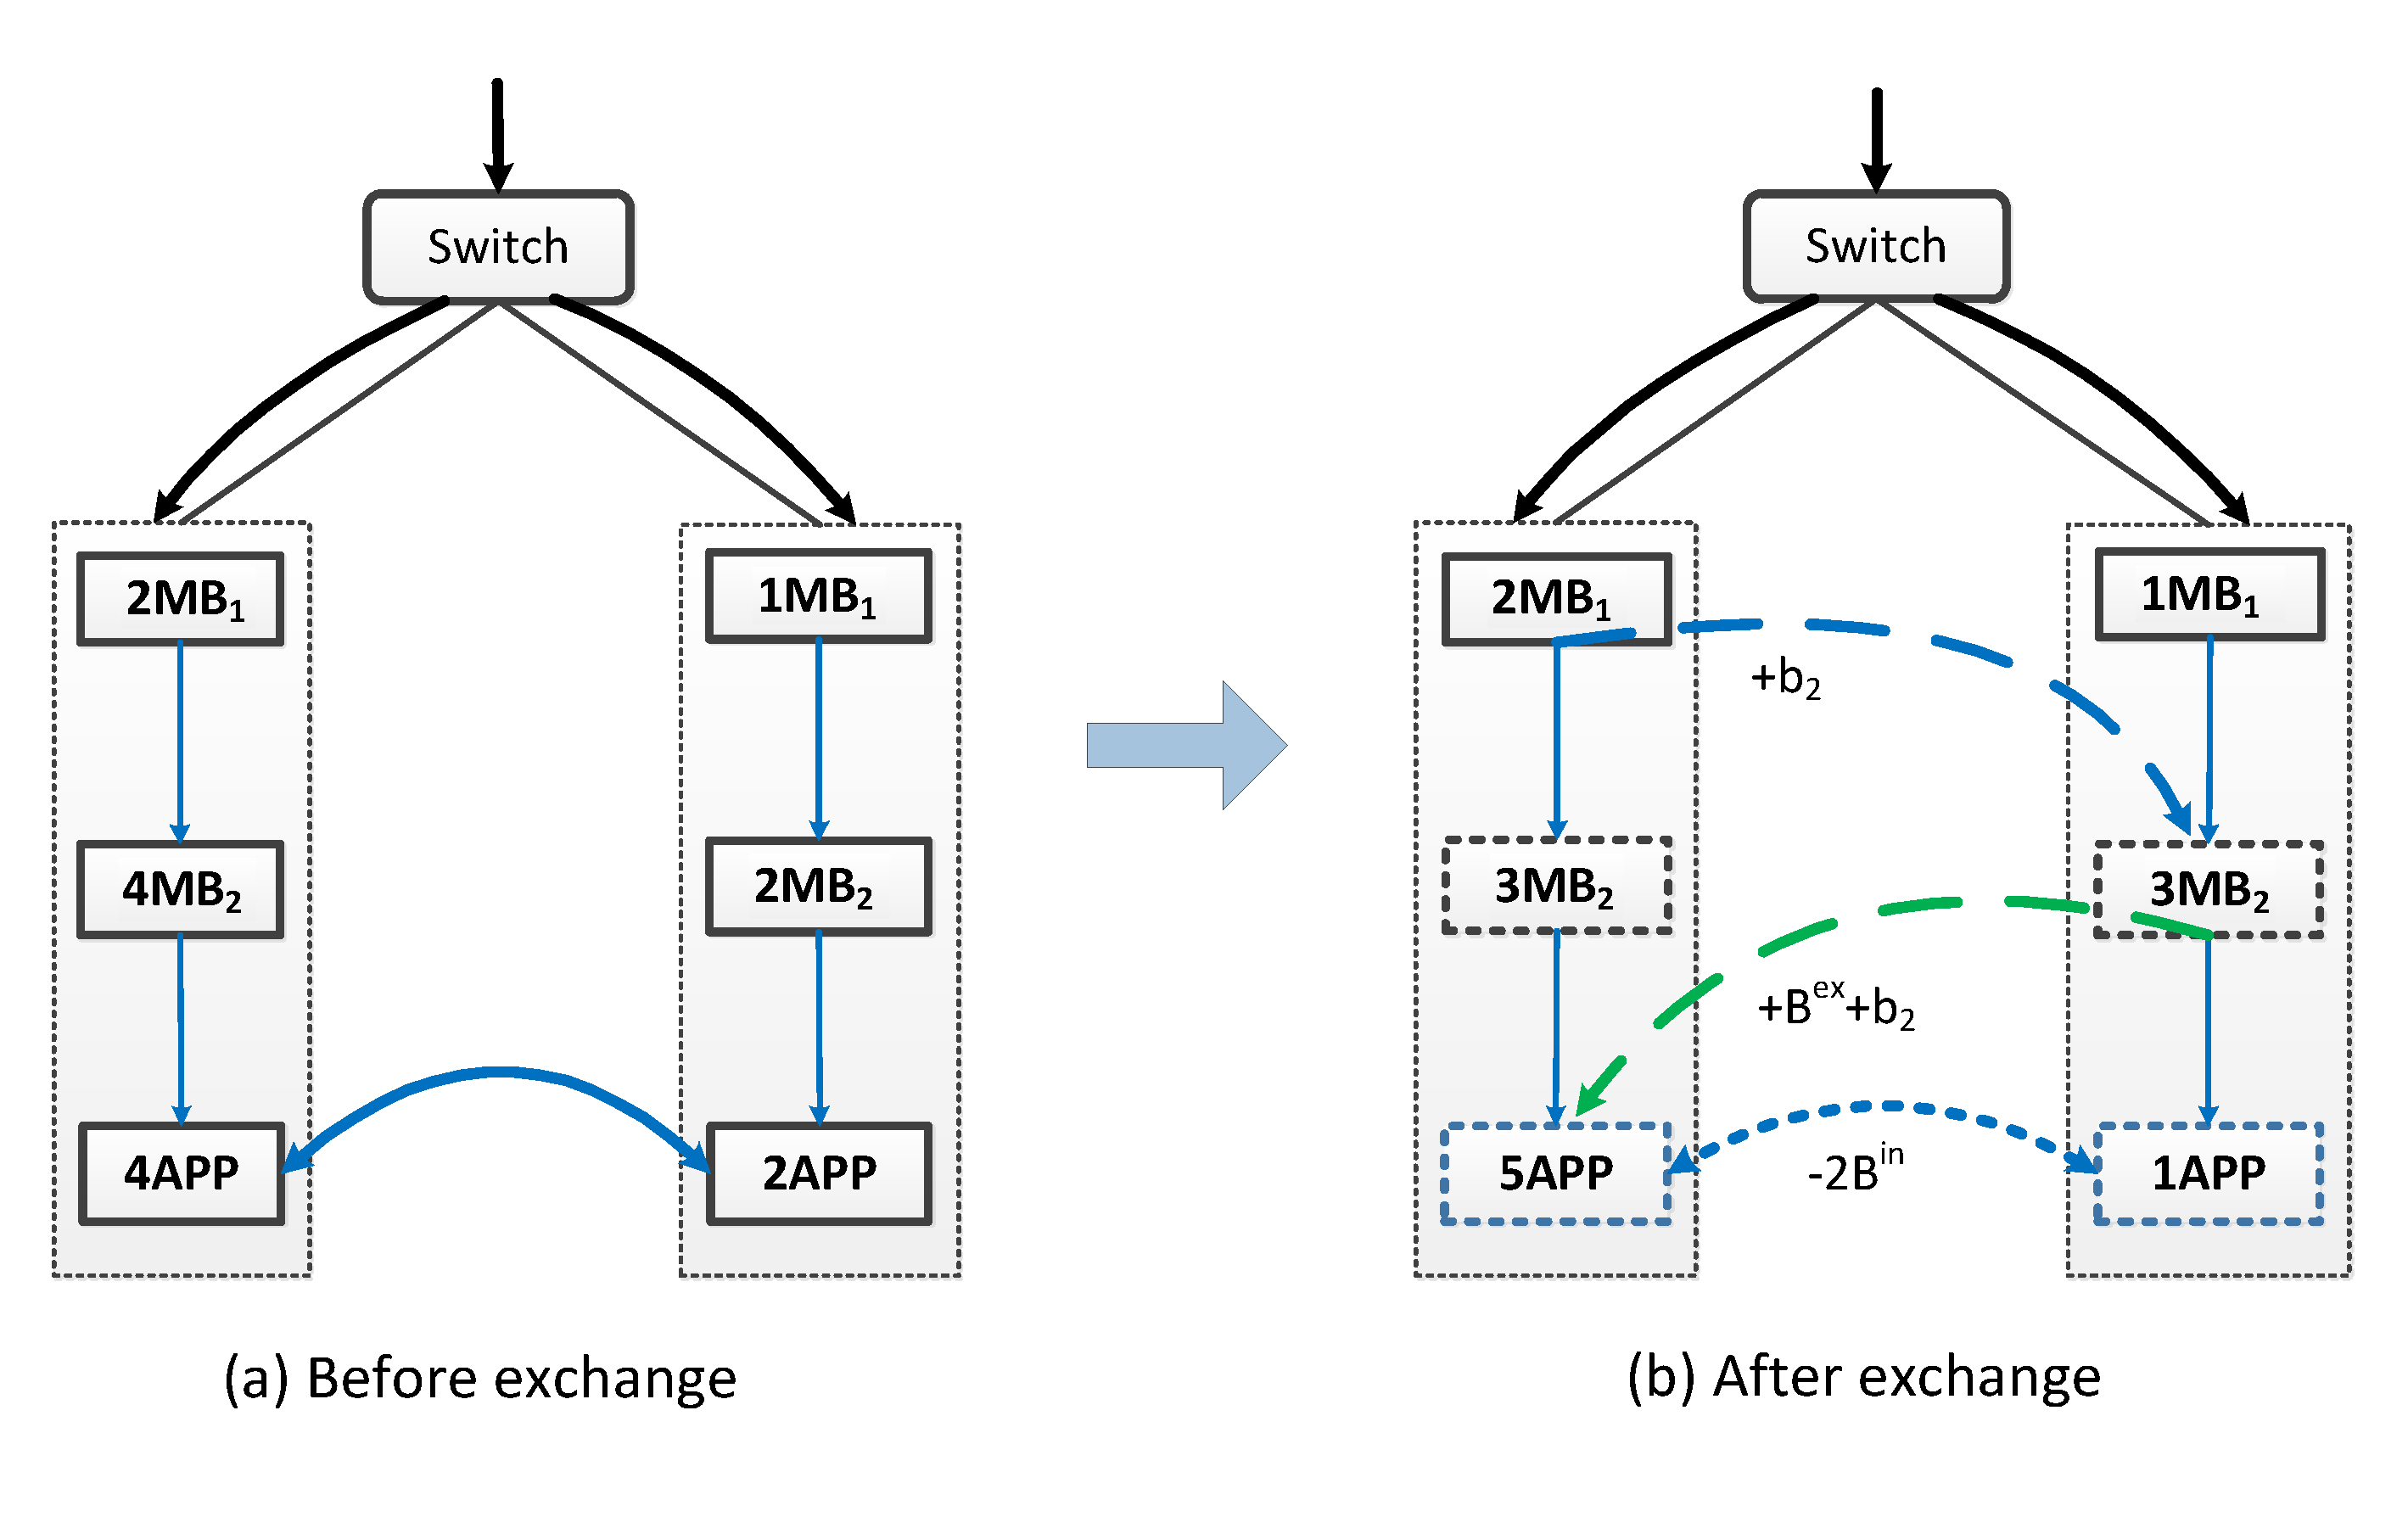
\includegraphics[width=3.5in]{fig/exchange_example.pdf}
	\caption{Illustration of the bandwidth variation after exchange}
    \label{fig:exchange}
\end{figure}
The exchange can break the proportion of the capacity of MBs and application, which will cause extra flows from one side to the other side and increase the bandwidth demands across the subtrees. On the other hand, we can increase the colocated APPs by exchanging, which will greatly reduce the intra-tenant bandwidth requirement. We let $C_1$ represents the increased portion of bandwidth due to the break of balanced capacity assignment, and $C_2$ denote the decreased portion of bandwidth caused by increasing the number of colocated APPs. If $C_1>C_2$, we say the portion of bandwidth reduction by colocating APPs is not able to make up for the cost of increased portion. The total bandwidth requirement then have an increase of $C_1-C_2$. However, if $C_1<C_2$, there will be much benefits to exchange since the total bandwidth cost will have a reduction of $C_2-C_1$. Therefore, the total bandwidth consumption may have an increase or decrease after the exchange.
%We then analyze the change of the bandwidth before and after the exchange of the MB and APP. 

For a more intuitive understanding of above results, consider a simple example as shown in Fig. \ref{fig:exchange}. The tenant request has been placed in two subtrees proportionally according to the placement step 1 showed in Fig. \ref{fig:exchange} (a). So the bandwidth requirements $B_{mb_k,mb_{k+1}}$ and $B_{mb,app}$ are almost zero since the traffic from $MB_k$ can be fully processed by $MB_{k+1}$s or APPs in the same subtree. Note that the number of APPs in the left subtree is larger than the number in the right side. We then try to exchange the $MB_2$ in the left side and APP in the right side to reduce the traffic across the subtrees between APPs. The result of exchange is shown in Fig. \ref{fig:exchange} (b). The dashed arrows show the change of traffic after exchange. The label associated with each arrow is the value of traffic change. %and the plus and minus signs indicate the increase or decrease for the change respectively.
 The long-dashed arrows show the increased portion of the bandwidth in the two links. While the short-dashed arrow represents the decreased portion of bandwidth across the subtrees. After the exchange, the $MB_2$ in the left side cannot totally handle the traffic from $MB_1$ in the same side. This leads to an extra flow from $MB_1$ in the left to $MB_2$ in the right side expressed in the blue long-dashed arrow. Similarly, the APPs in the left side get additional capacity to process the extra flow from $MB_2$ in the right side due to the exchange showed by the green long-dashed arrow. For the intra-tenant communication, we get a decrease of bandwidth represented by the short-dashed arrow through increasing the number of colocated APPs in one side. Clearly, in this example, $C_1$ is equal to the sum of the two extra flows' bandwidth requirements computed as $b_2+(b_2+B^{ex})=2b_2+B^{ex}$, where $b_2$ is the practical required capacity of $MB_2$ defined by Eq. \ref{equ:bk}. And $C_2$ is equal to $2B^{in}$ which is the bandwidth saving of intra-tenant communication. 

Thus, if $C_2>C_1$ or $2B^{in} > 2b_2 + B^{ex}$, it is a better choice to exchange, i.e., the total bandwidth consumption in the two links will be reduced if the decreased portion is larger than the increased portion of the bandwidth after the exchange. And, we can easily get the following exchange conditions for any $MB_k$ using the same analyzing method as shown above: 
\begin{equation}
\begin{aligned}
&2B^{in}>b_k+B^{ex},k=1;\\
&2B^{in}>2b_k+B^{ex},k>1.
\end{aligned}
\end{equation}

However, we currently only consider the total bandwidth variation of the two links. For the single link, there may be a different result, i.e., the total decrease of the bandwidth cannot ensure that both of the links have a reduction of bandwidth. For a better understanding, we assume $b_2 = 200$, $B^{ex} = 600$, and $B^{in} = 502$ (in Mbps). Explicitly, $MB_2$ satisfies the exchange condition mentioned above. Consider the simple example shown in Fig. \ref{fig:exchange}. The right link get a bandwidth reduction computed as $B^{in}-b_2=502-200=302$ Mbps after exchange. While the left link have a bandwidth increase of $(B^{ex}+b_2)-B^{in}=600+200-502=298$ Mbps. So the total bandwidth has been reduced. But the exchange may lead to an unbalanced utilization of the two links. And the tenant request will be rejected if the remain bandwidth is smaller than 298 Mbps in the left link before the exchange. To avoid this situation, we reconsider the condition of exchange to ensure that both links have bandwidth savings. As shown in Fig. \ref{fig:exchange}, the two links both get an extra traffic flow which causes a bandwidth increase ($b_2$ and $B^{ex}+b_2$ respectively) from the opposite side, respectively. In addition, there is a bandwidth reduction of $B^{in}$ for intra-tenant communication in both of the links. Further, for the left link, there is a bandwidth variation $C_l=B^{ex}+b_2-B^{in}$. While for the right link, the bandwidth variation is $C_r=b_2-B^{in}$. If $C_l<0$ (or $C_r<0$), the bandwidth demand will be reduced in the left link (or right link). Thus, the condition to have bandwidth savings for both links is given as
\begin{equation}
\begin{aligned}
%B^{in}-(B^{ex}+b_2)>0 \quad and \quad B^{in}-b_2>0,
&C_l<0 \quad and \quad C_r<0 \quad or \\
&B^{ex}+b_2<B^{in} \quad and \quad b_2<B^{in}.
\end{aligned}
\end{equation}
i.e., if $B^{in}>(B^{ex}+b_2)$, the bandwidth will be saved for both of the links. Similarly, we can easily obtain the following improved conditions to get a more proper exchanging for any middlebox $MB_k$. 
\begin{equation}
\begin{aligned}
&B^{in}>b_k\quad and \quad B^{in}>B^{ex}, k=1;\\
&B^{in}>b_k+B^{ex}, k>1.
\end{aligned}
\label{equ:condition}
\end{equation}

Thus, using the improved exchangeable conditions to select the proper type of middleboxes for exchanging \footnote{Equ. \ref{equ:condition} is a sufficient but not necessary condition for bandwidth saving through exchanging, and we can also have bandwidth saving even the VMs are placed randomly initially by exchanging using Equ. \ref{equ:condition}.},
	%\begin{comment}and we currently only consider one type of middlebox for exchanging at a time. While it may achieve a larger bandwidth saving by exchanging two or more different types of middleboxes simultanously. We leave this for future work.},\end{comment}}
we cannot achieve a total bandwidth saving but ensuring a bandwidth reduction for each of the links when placing the tenant request.


\subsection{VM Placement Algorithm}

Based on above placement principles and exchangeable conditions, we design an effective heuristic VM placement algorithm that achieves bandwidth savings while providing guarantees. The basic idea behind the algorithm is to place MBs and APPs proportionally initially to minimize the bandwidth consumption due to the unbalanced capacity assignment between middleboxes and application VMs; and then try to colocate more APPs to reduce the bandwidth cost of intra-tenant communication through exchanging MBs and APPs. 

The algorithm starts with $PlaceTenant$ (line 1), which takes a tenant request t as an input. To save the precious core level bandwidth, we traverse the datacenter topology in a bottom-up manner to search for a valid lowest level subtree that has enough VM slots for t (line 2). For the candidate subtree, we place t in it with $AllocateVM$ (line 4) and then check whether the bandwidth requirement can be satisfied (line 5). If the trial fails due to the lack of bandwidth, $DeAllocate$ (line 7) is invoked to release the resources reserved for the tenant request. And the algorithm continues to find another subtree in the same level or upper level if there is no subtree in the same level (line 8). 
\begin{algorithm}[!htbp]
	\caption{VM Placement Algorithm}
	\label{alg1}
	\begin{algorithmic}[1]
		\Function{PlaceTenant}{Tenant t}
		\State st = FindlowestSubtree(t, null)
		\While{st}
		   \State AllocateVM(t, t.mb, t.app, st)
		   \If{ReserveBw(t)}
			   \State return true
		   \EndIf 
		   \State DeAllocate(t)
		   \State st = FindLowestSubtree(t, st)
%		   \If {st is null}
%			   \State return false
%		   \EndIf
		\EndWhile
		\State return false
%		\State
	  \EndFunction
	  \Function{AllocateVM}{t, $N_{mb}$, $N_{app}$, st}\\
	  /*$N_{mb}$ stores the number of instances for each type of middleboxes, while $N_{app}$ is the number of application VMs.*/
	  \If {level(st)==0} /*st is a server*/
		  \State PlaceMB(t, $N_{mb}$, st)
		  \State PlaceAPP(t, $N_{app}$, st)
	  \Else
	  \For {each subtree v of st}
		  \If{AvailableVM(v)$>$0}
			  \If{AvailableVM(v)$<$TotalVM($N_{mb}$,$N_{app}$)}
				  \State place $N_{v\_mb}$MBs and $N_{v\_app}$APPs \State proportionally under v.
				  \State $N_{mb} = N_{mb} - N_{v\_mb}$
				  \State $N_{app} = N_{app} - N_{v\_app}$
				  \State ExchangeMbApp($N_{mb}$,$N_{app}$,$N_{v\_mb}$,$N_{v\_app}$)
				  \State AllocateVM(t, $N_{v\_mb}$, $N_{v\_app}$, v)
		      \Else
			      \State AllocateVM(t, $N_{mb}$, $N_{app}$, v)
			  \EndIf
		\EndIf
	  \EndFor
	\EndIf
   \EndFunction %\\
   \Function{ExchangeMbApp}{$N_{mb}$,$N_{app}$,$N_{v\_mb}$,$N_{v\_app}$}
	   \State mb = GetExchangeableMB(t)
	   \If{mb!=null}
	       \State $num$ is assigned as the number of types
	       \State of the exchangeable MBs.
	       \State $k = 0$
		   \If{$N_{app}>N_{v\_app}$}
		     \While{$k<num \quad and\quad N_{v\_app}!=0$} 
			   \If{$N_{mb}[mb[k]]==0$}
				   \State $k$++
				   \State $continue$
			   \EndIf
			   \State $N_{mb}[mb[k]]$- -
			   \State $N_{app}$++
		 	   \State $N_{v\_mb}[mb[k]]$++
			   \State $N_{v\_app}$- -
			\EndWhile
	    \Else
	      \While{$k<num \quad and \quad N_{app}!=0$}
		    \If {$N_{v\_mb}[mb[k]]==0$}
			   \State $k$++
			   \State $continue$
			\EndIf
			\State $N_{v\_mb}[mb[k]]$- -
			\State $N_{v\_app}$++
			\State $N_{mb}[mb[k]]$++
			\State $N_{app}$- -
		 \EndWhile
	   \EndIf
	  \EndIf
   \EndFunction    
  \end{algorithmic}
   
\end{algorithm}		

 $AllocateVM$ (line 10) is a recursive function, which takes a tenant request t, its APP and MB VMs’ number and a subtree st as inputs. The function first checks if the st is the lowest level subtree or physical server: if so, it allocates corresponding number of slots for t according to the parameters of $N_{app}$ and $N_{mb}$ in the server and then returns. If st is a higher level switch, we then invoke $AllocateVM$ recursively for each subtree v of st which has available VM slots. For the subtree v that cannot provide enough slots for the unallocated MB and APP VMs, we first attempt to place appropriate number of MBs and APPs according to the placement principle1 to fill the subtree v and then colocate as many APPs as possible by exchanging MBs and APPs using the exchangeable conditions of Equ. \ref{equ:condition} . After that, we invoke the function $AllocateVM$ (line 24) for the ajusted MB and APPs. While for the subtree of st that has sufficient slot resource, AllocateVm is invoked directly (line 26). 

%The function exchangeMbApp is invoked to exchange the positions of MBs and APPs. 
$ExchangeMbApp$ (line 27) is invoked to exchange the positions of MBs and APPs. The function first identifies the types of middleboxes that can achieve bandwidth saving through exchanging their and APPs’ positions by using the exchangeable conditions of Eq. \ref{equ:condition}. If the exchangeable middleboxes exist, we then check the number of APPs in the two subtrees and exchange the smaller one with the MBs to increase the degree of colocation for APPs. We excute the exchanging until all exchangeable MBs or APPs have been exchanged. If current exchangeable MBs have been exchanged completely, we then select the next exchangeable type of MBs to exchange (line 35). After each exchanging, we update the number of MBs and APPs in the two sides.
\begin{figure}
	\centering
	\subfigure[Accept rate under different $B^{in}$]{
	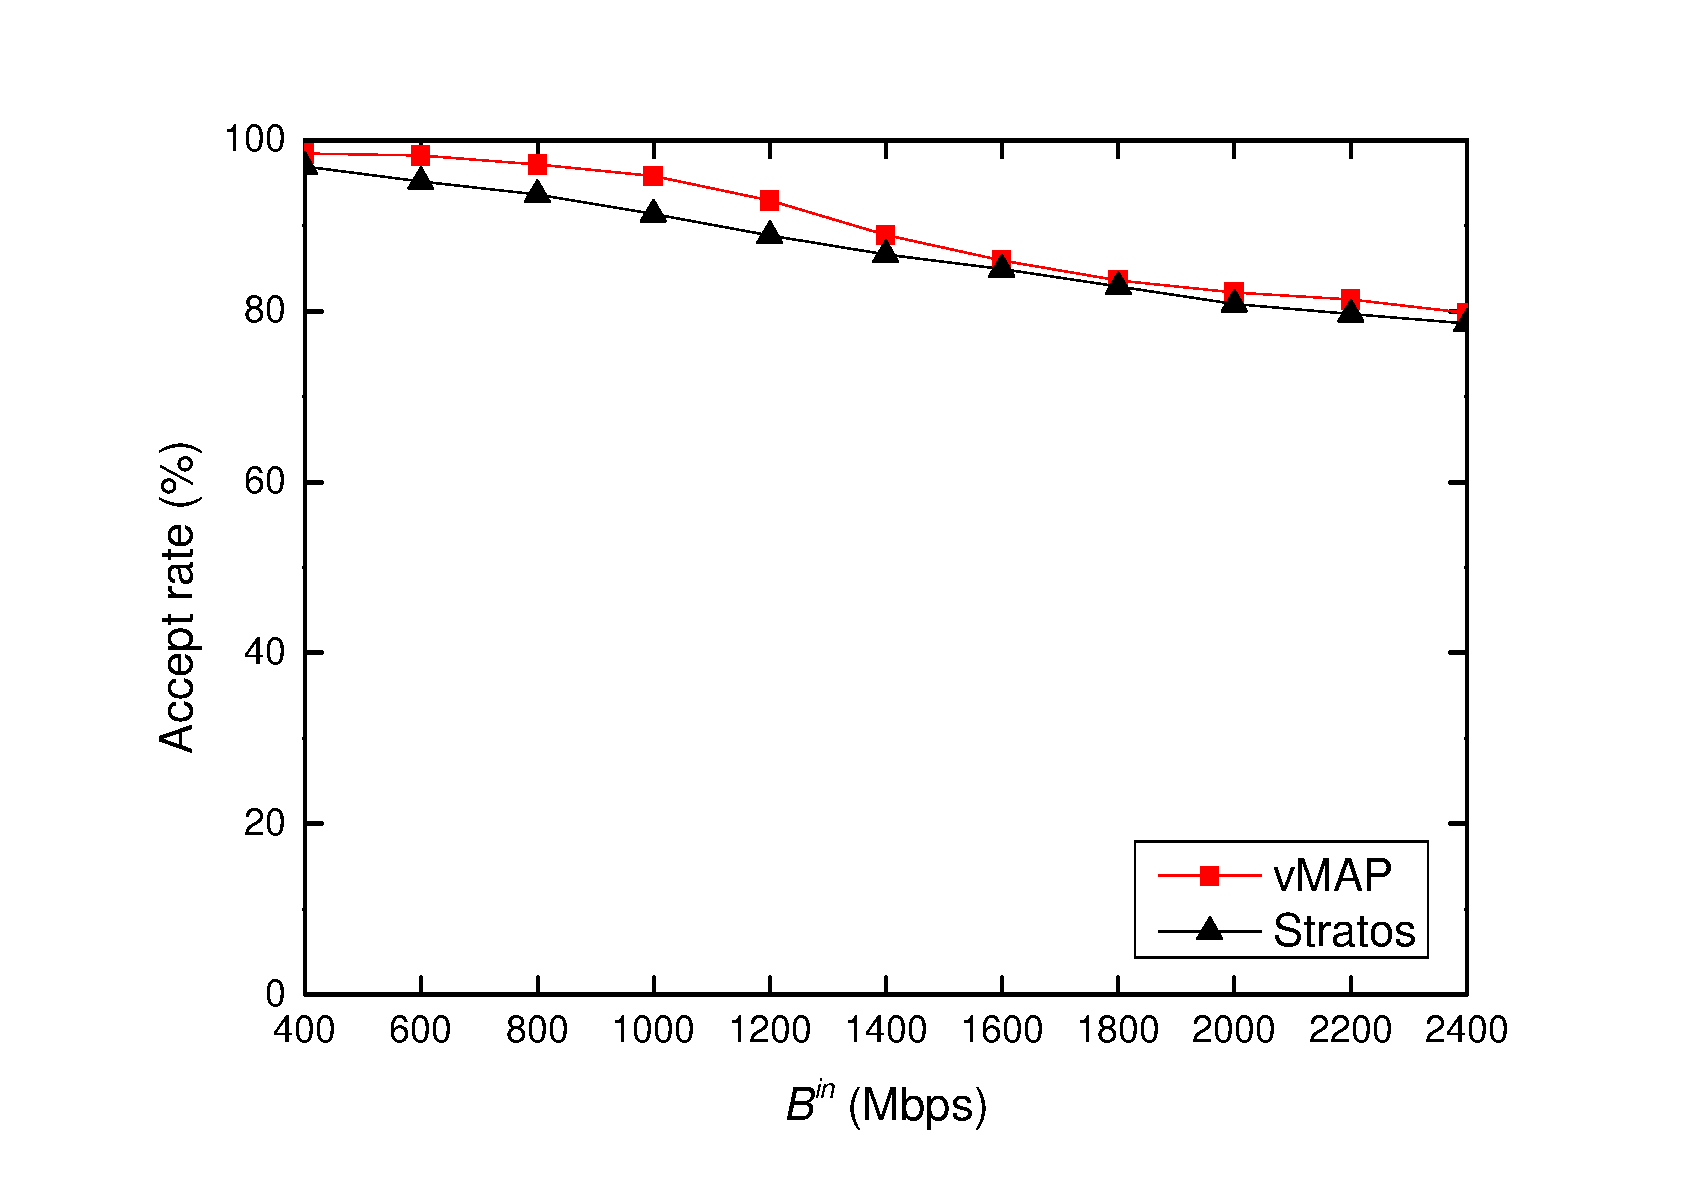
\includegraphics[width=3.2in,height=2.0in]{fig/accept_rate_bin.pdf}
	%\label{fig:accept_rate_bin}
	%\caption{Accept rate under different $B^{in}$}
	\label{fig:accept_rate_bin}}
	%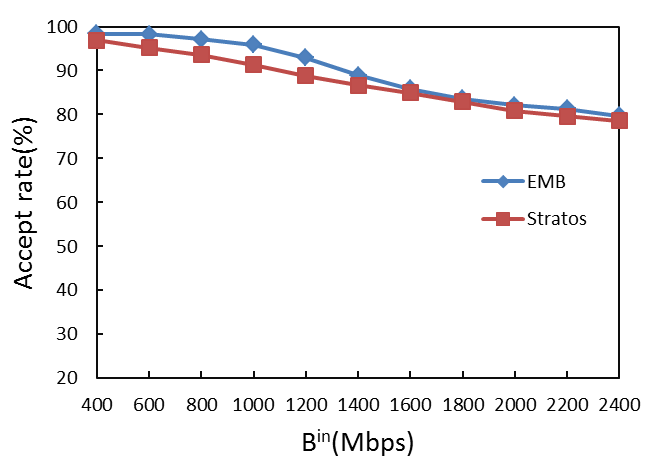
\includegraphics[width=3.2in]{fig/accept_rate_bin.png}
%\end{figure}

%\begin{figure}
	\subfigure[Accept rate under different $B^{ex}$]{
	\centering
	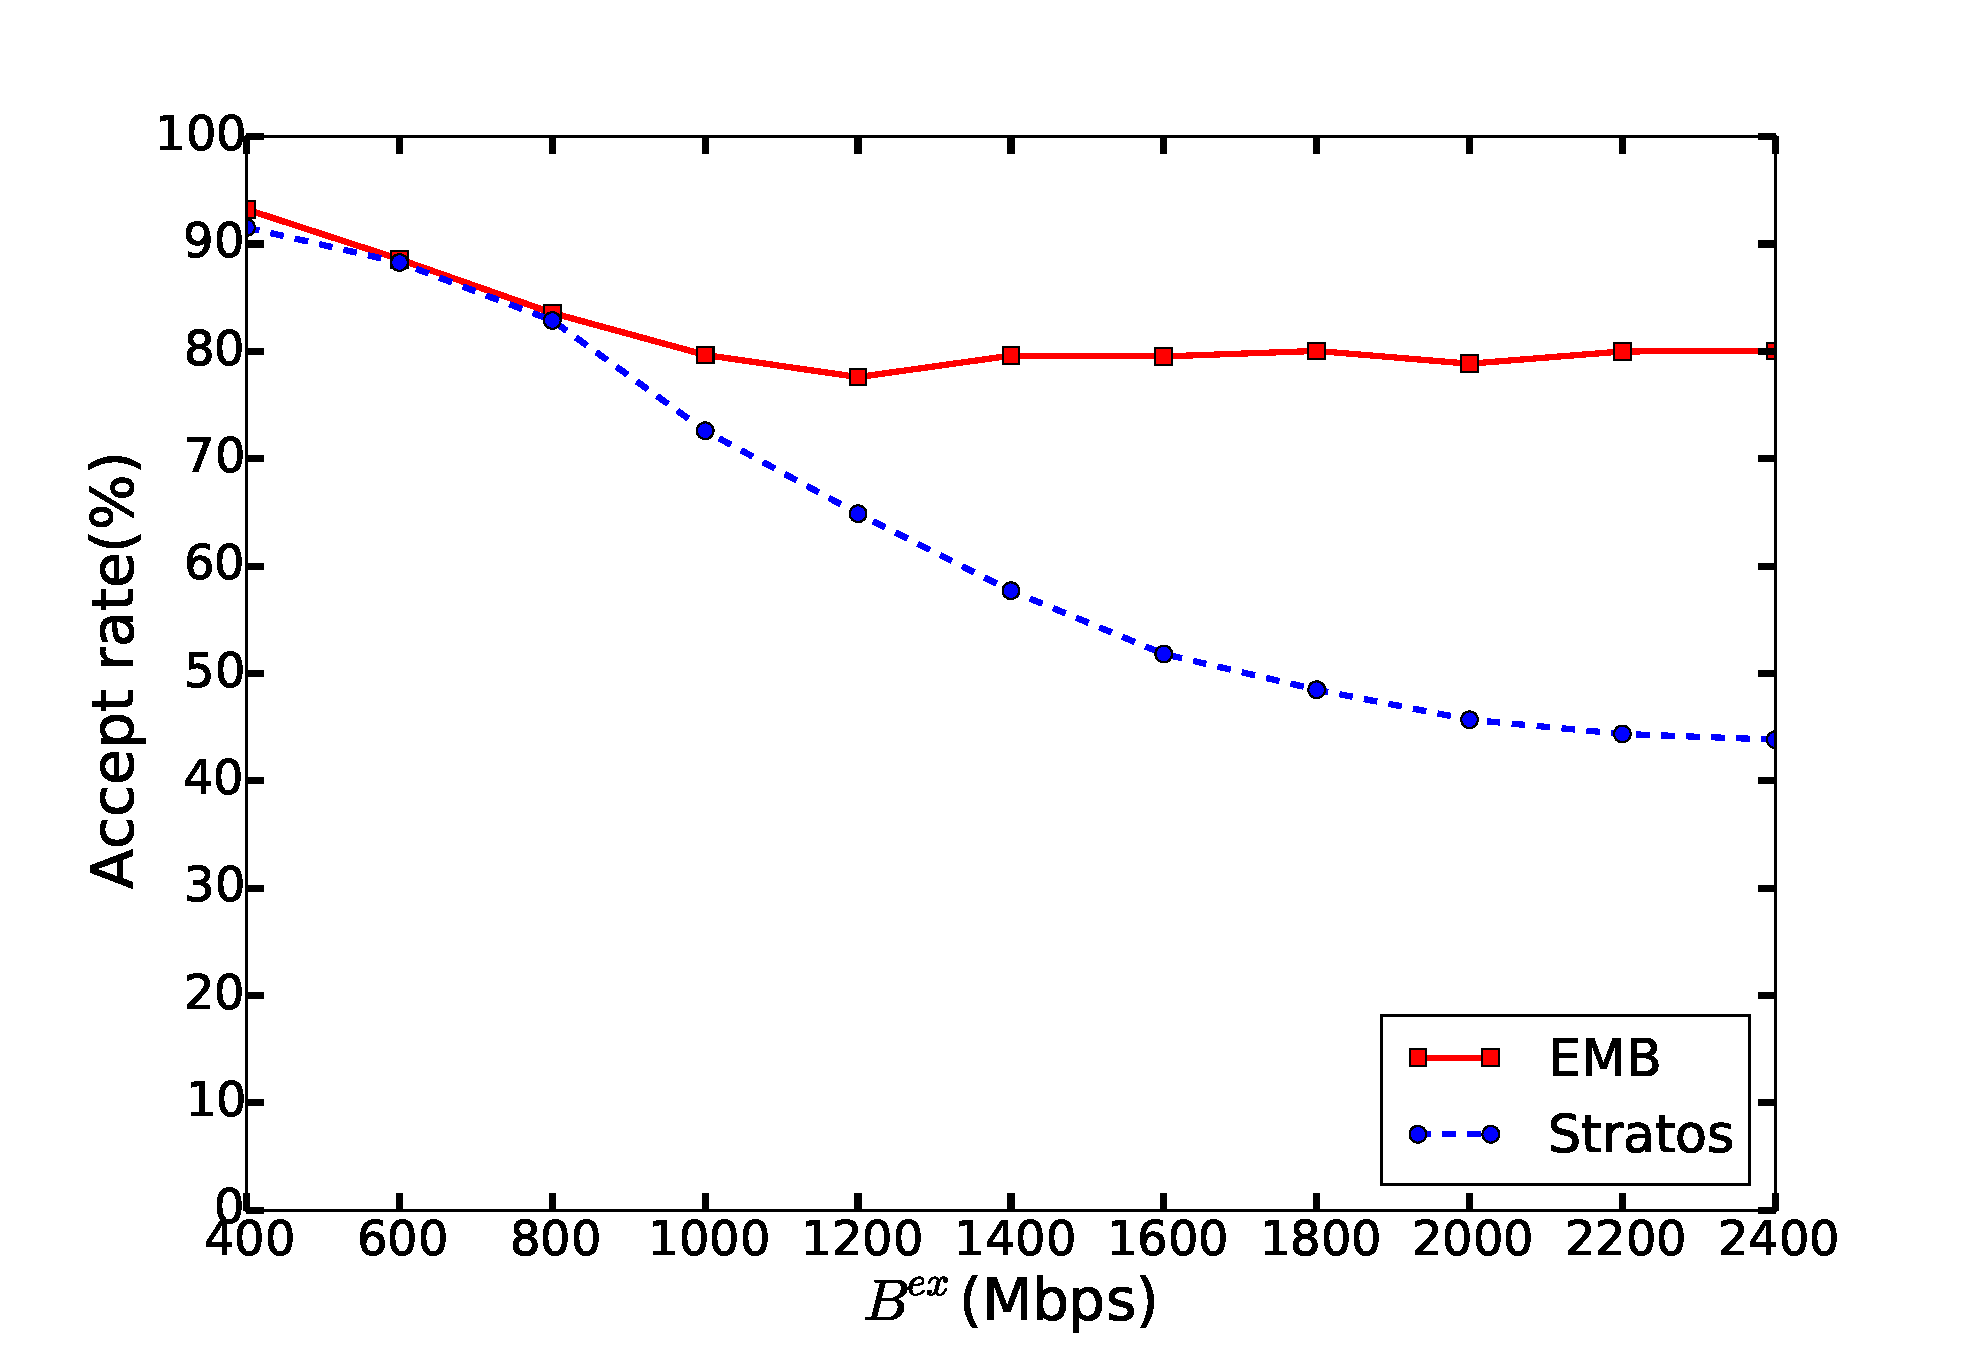
\includegraphics[width=3.2in,height=2.0in]{fig/accept_rate_bex.pdf}
	%\caption{Accept rate under different $B^{ex}$}
	\label{fig:accept_rate_bex}}
	\caption{Accept rate under different $B^{in}$ and $ B^{ex}$}
	\label{fig:accept_rate}
\end{figure}

\begin{figure}
	\centering
	
	\subfigure[VM slot utilization under different $B^{in}$]{
		\label{fig:vm_util_bin}
		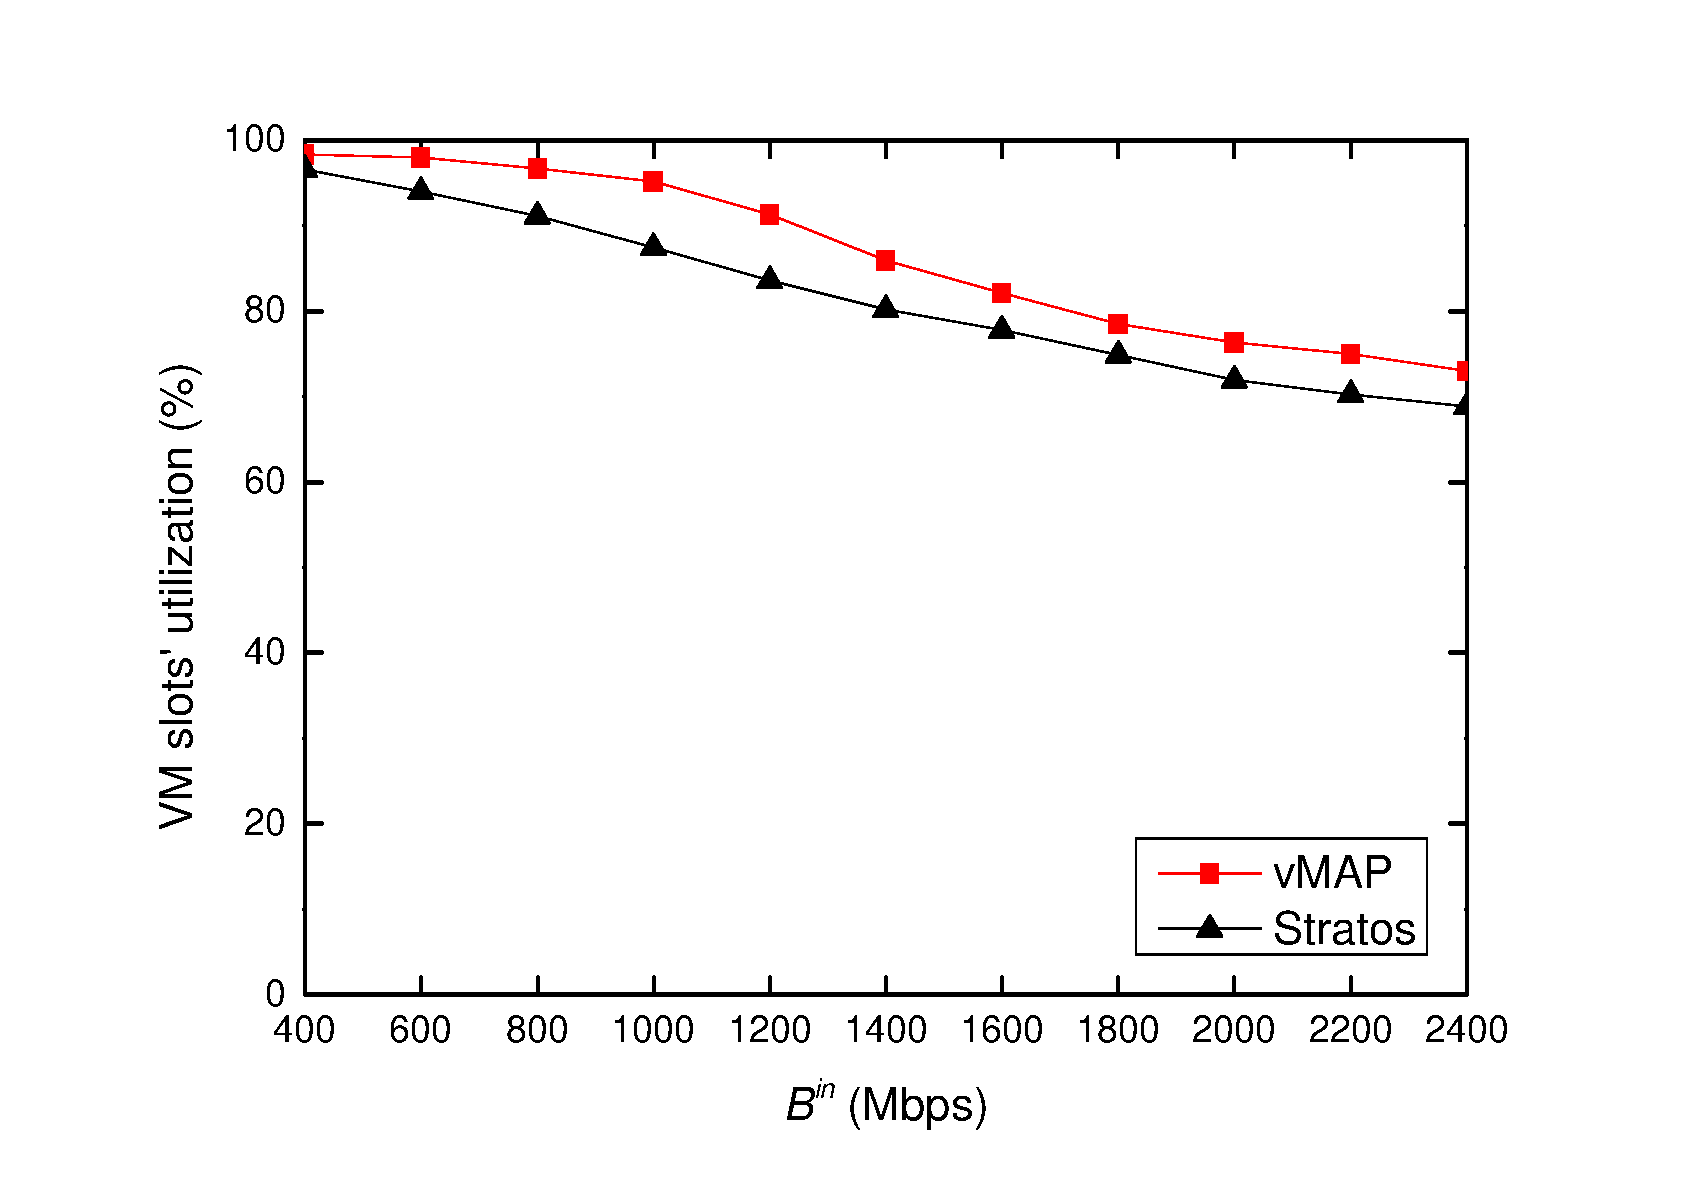
\includegraphics[width=3.2in, height=2.0in]{fig/vm_util_bin.pdf}
	}
	\subfigure[VM slot utilization under different $B^{ex}$]{
		\label{fig:vm_util_bex}
		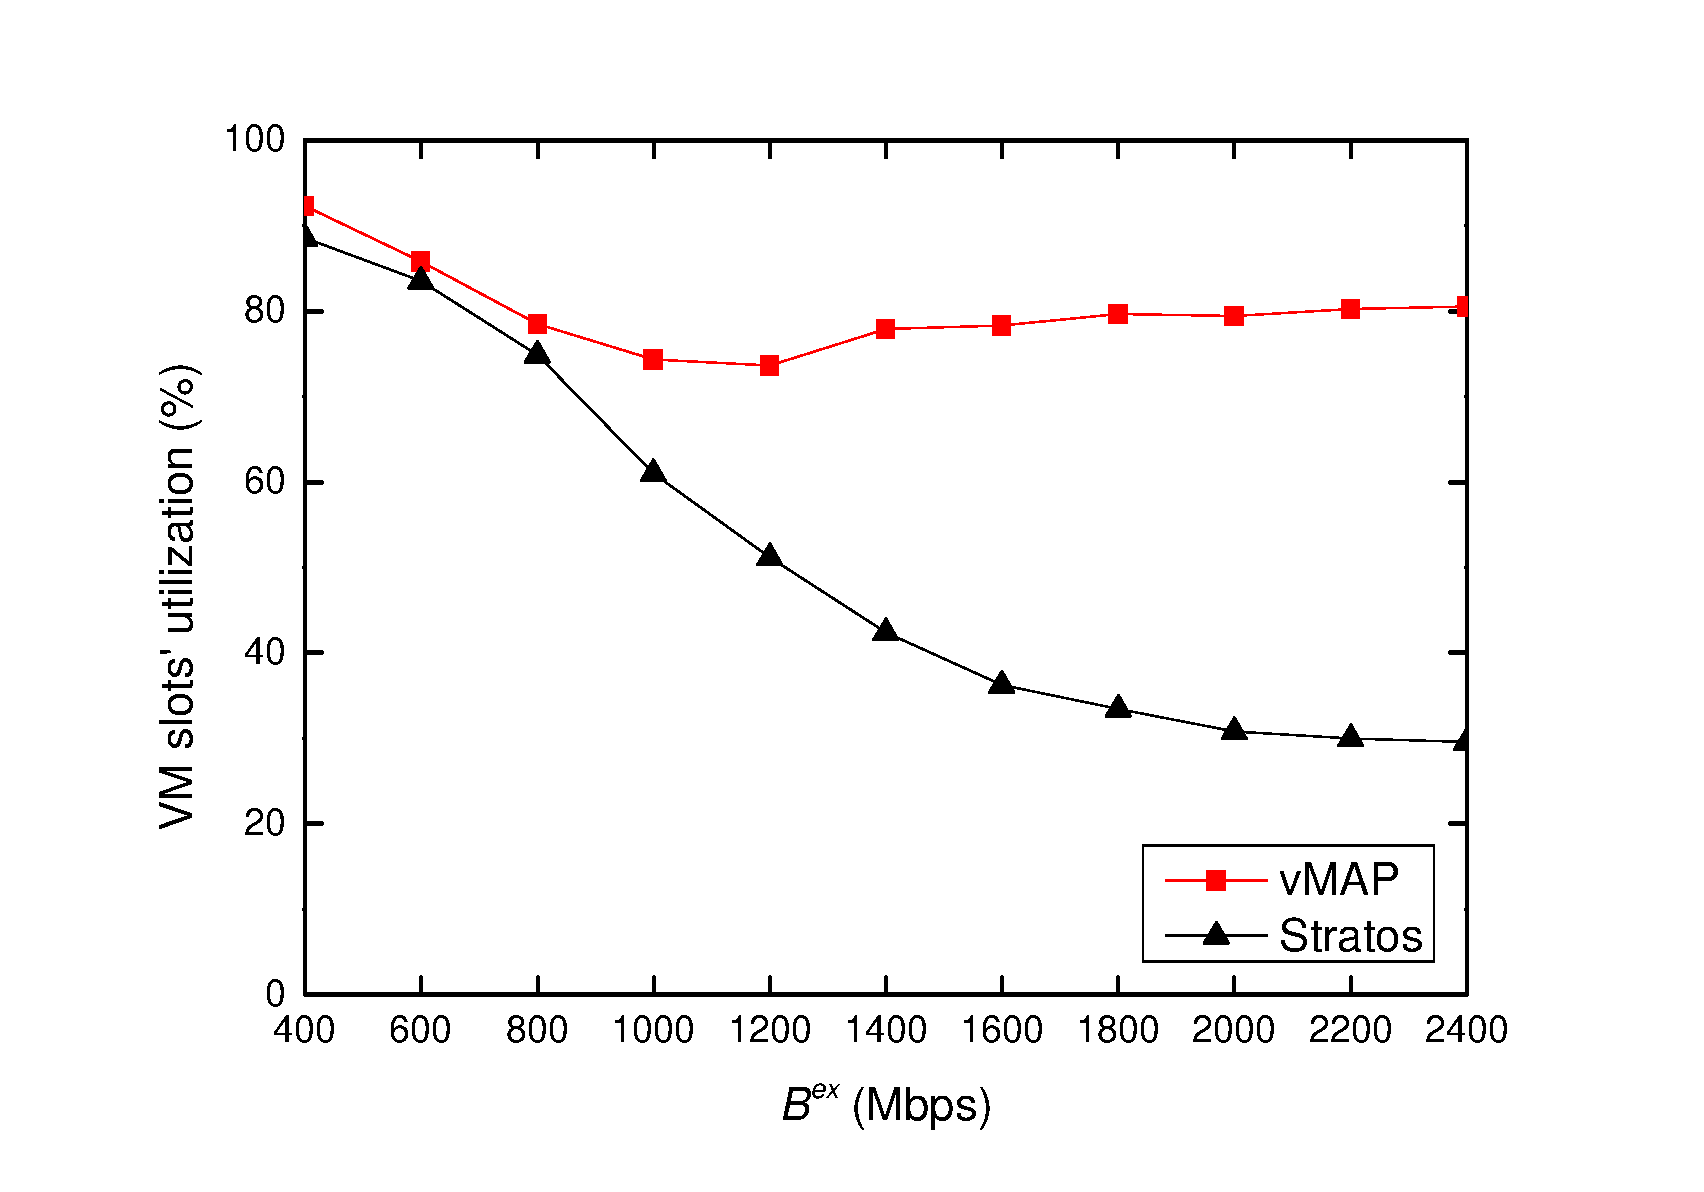
\includegraphics[width=3.2in, height=2.0in]{fig/vm_util_bex.pdf}
	}
	%\label{fig:vm_util}
	\caption{VM slot utilization under different $B^{in}$ and $B^{ex}$}
	\label{fig:vm_util}
\end{figure}

\begin{figure}
	\centering
	\subfigure[Core-aggregation links' bandwidth utilization]{
		\label{fig:agg_core}
		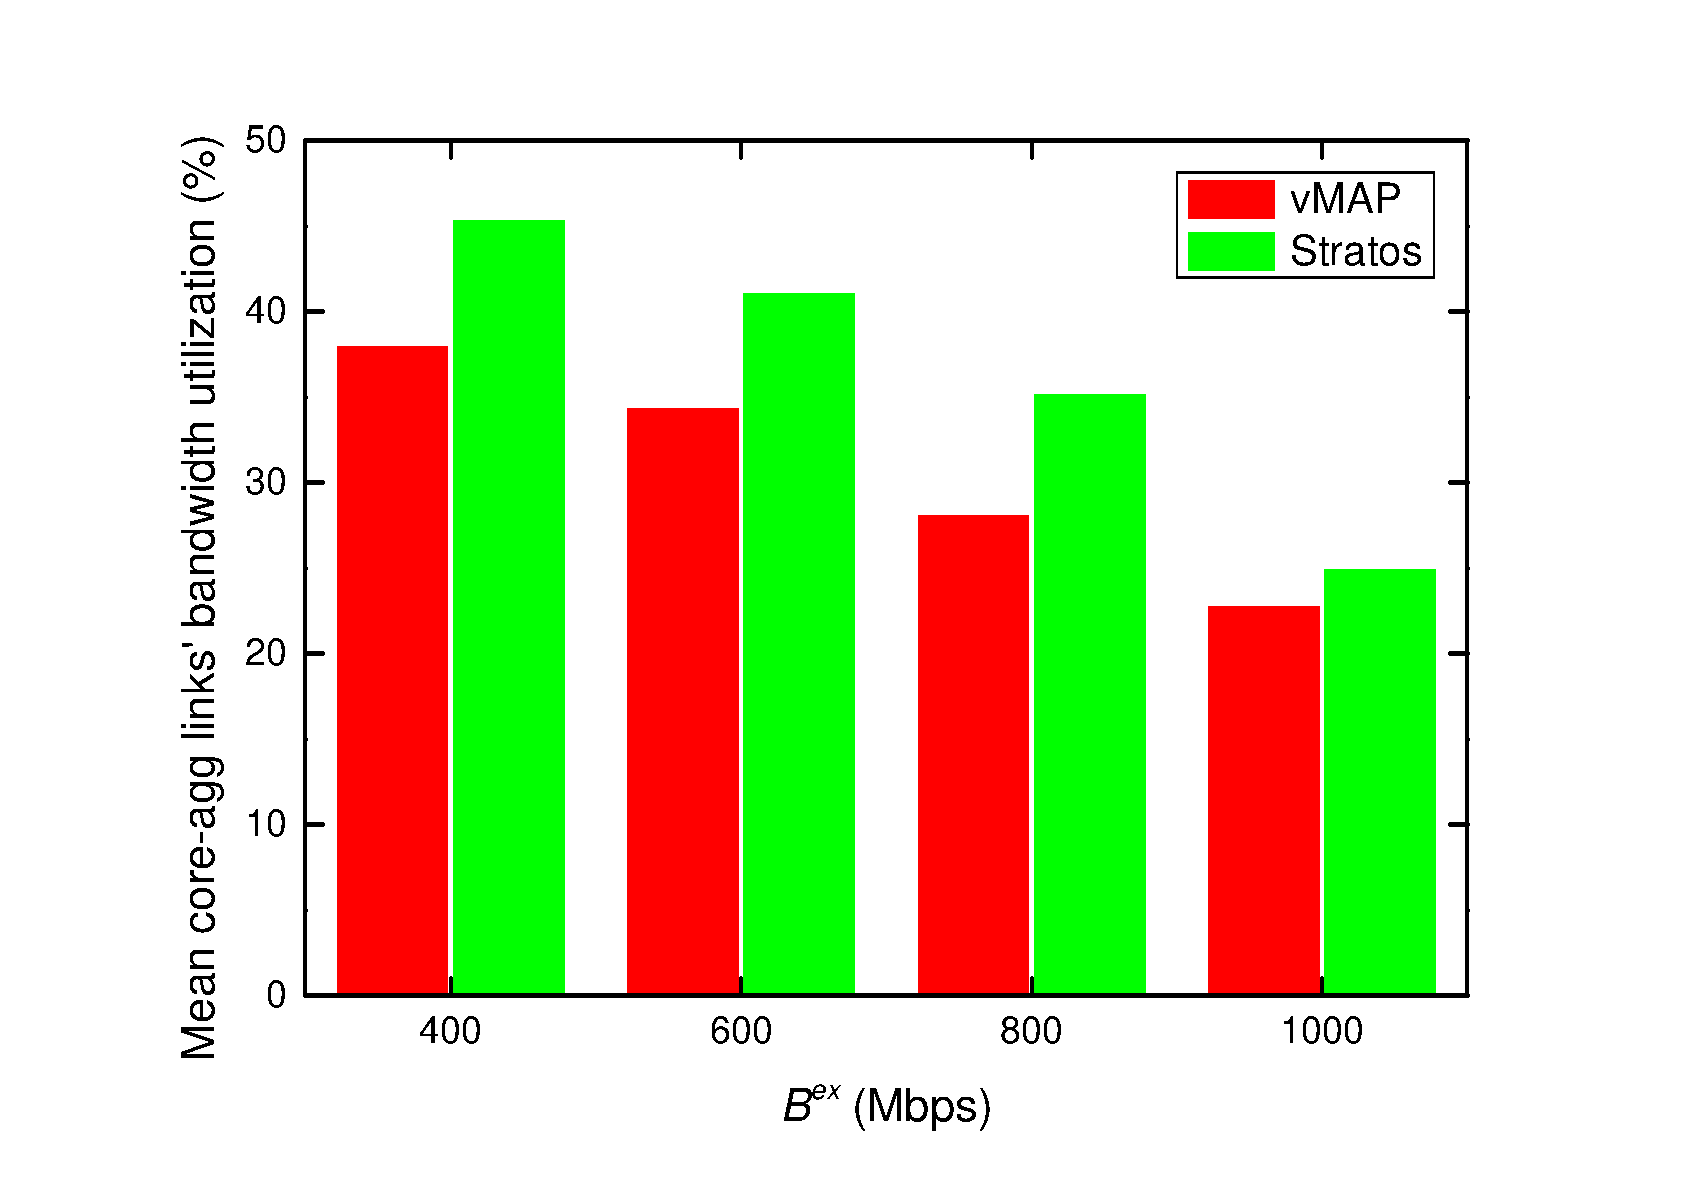
\includegraphics[width=2.4in]{fig/high_bw_util.pdf}}
	\subfigure[ToR-PM links' bandwidth utilization]{
		\label{fig:pm_agg}
		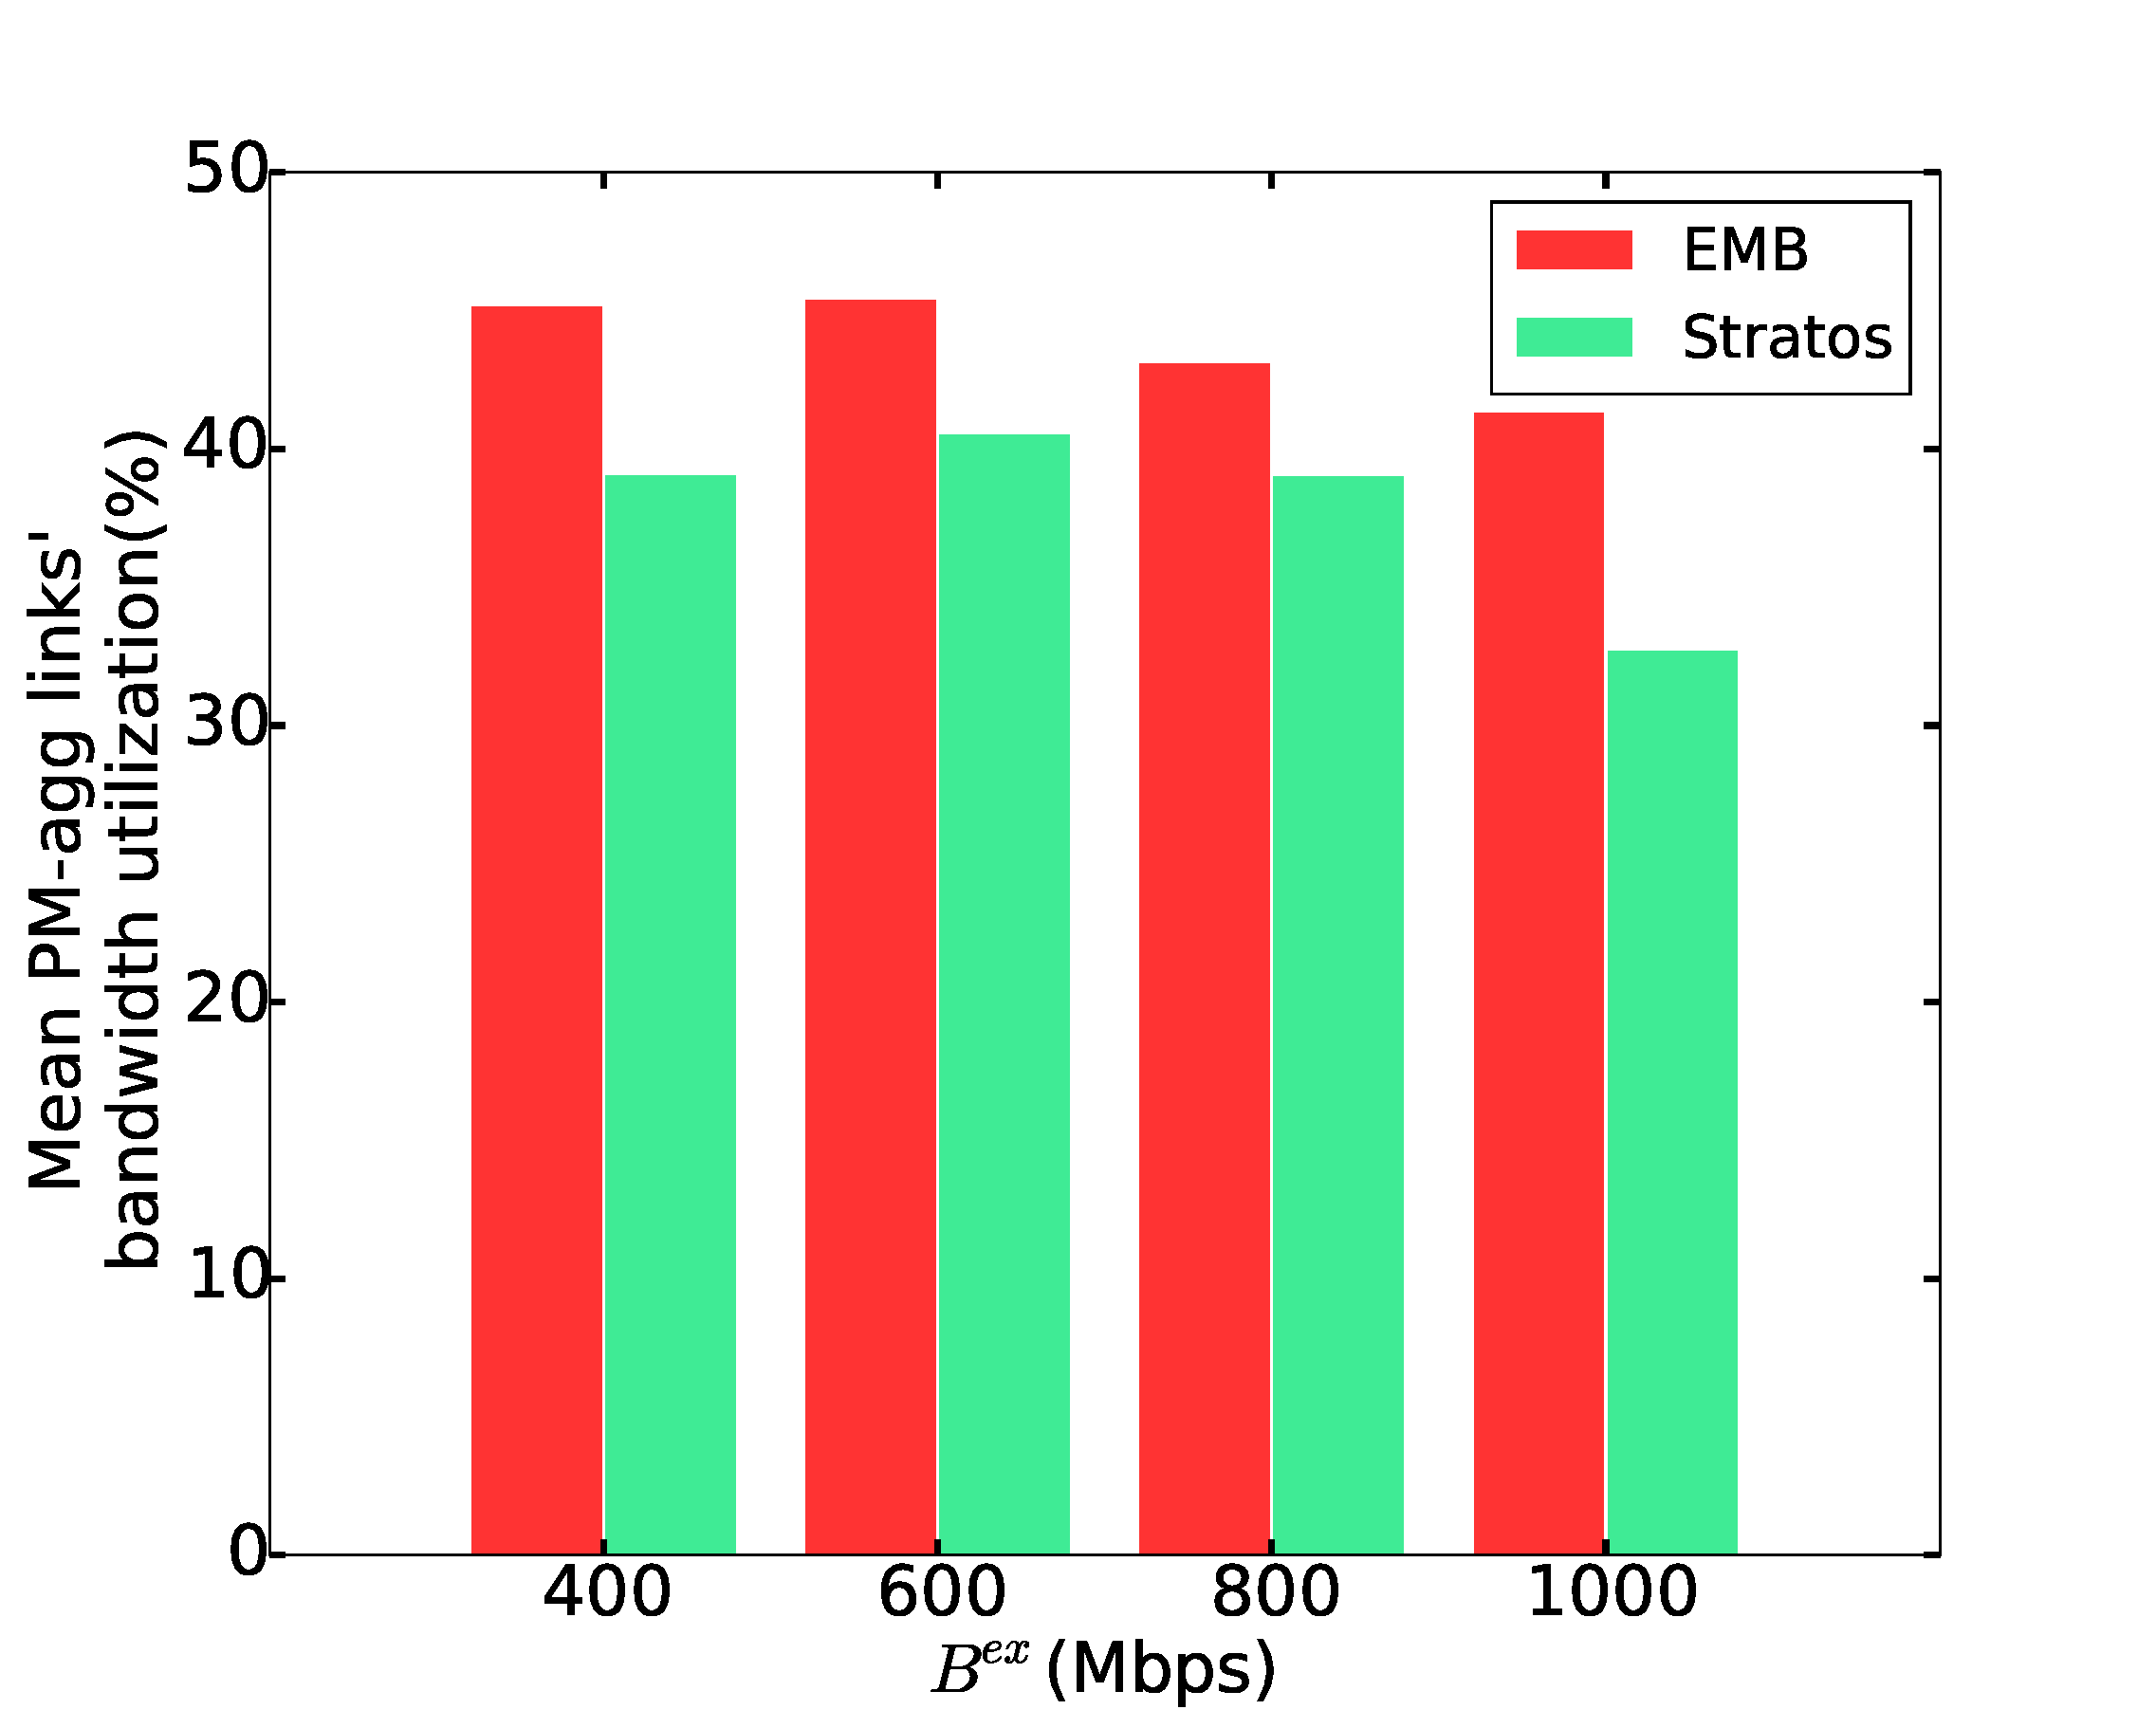
\includegraphics[width=2.5in]{fig/low_bw_util.pdf}}
	\caption{Bandwidth utilization under different $B^{ex}$}
	\label{fig:bw_util}
\end{figure}
\begin{comment}
\begin{figure}
	\centering
	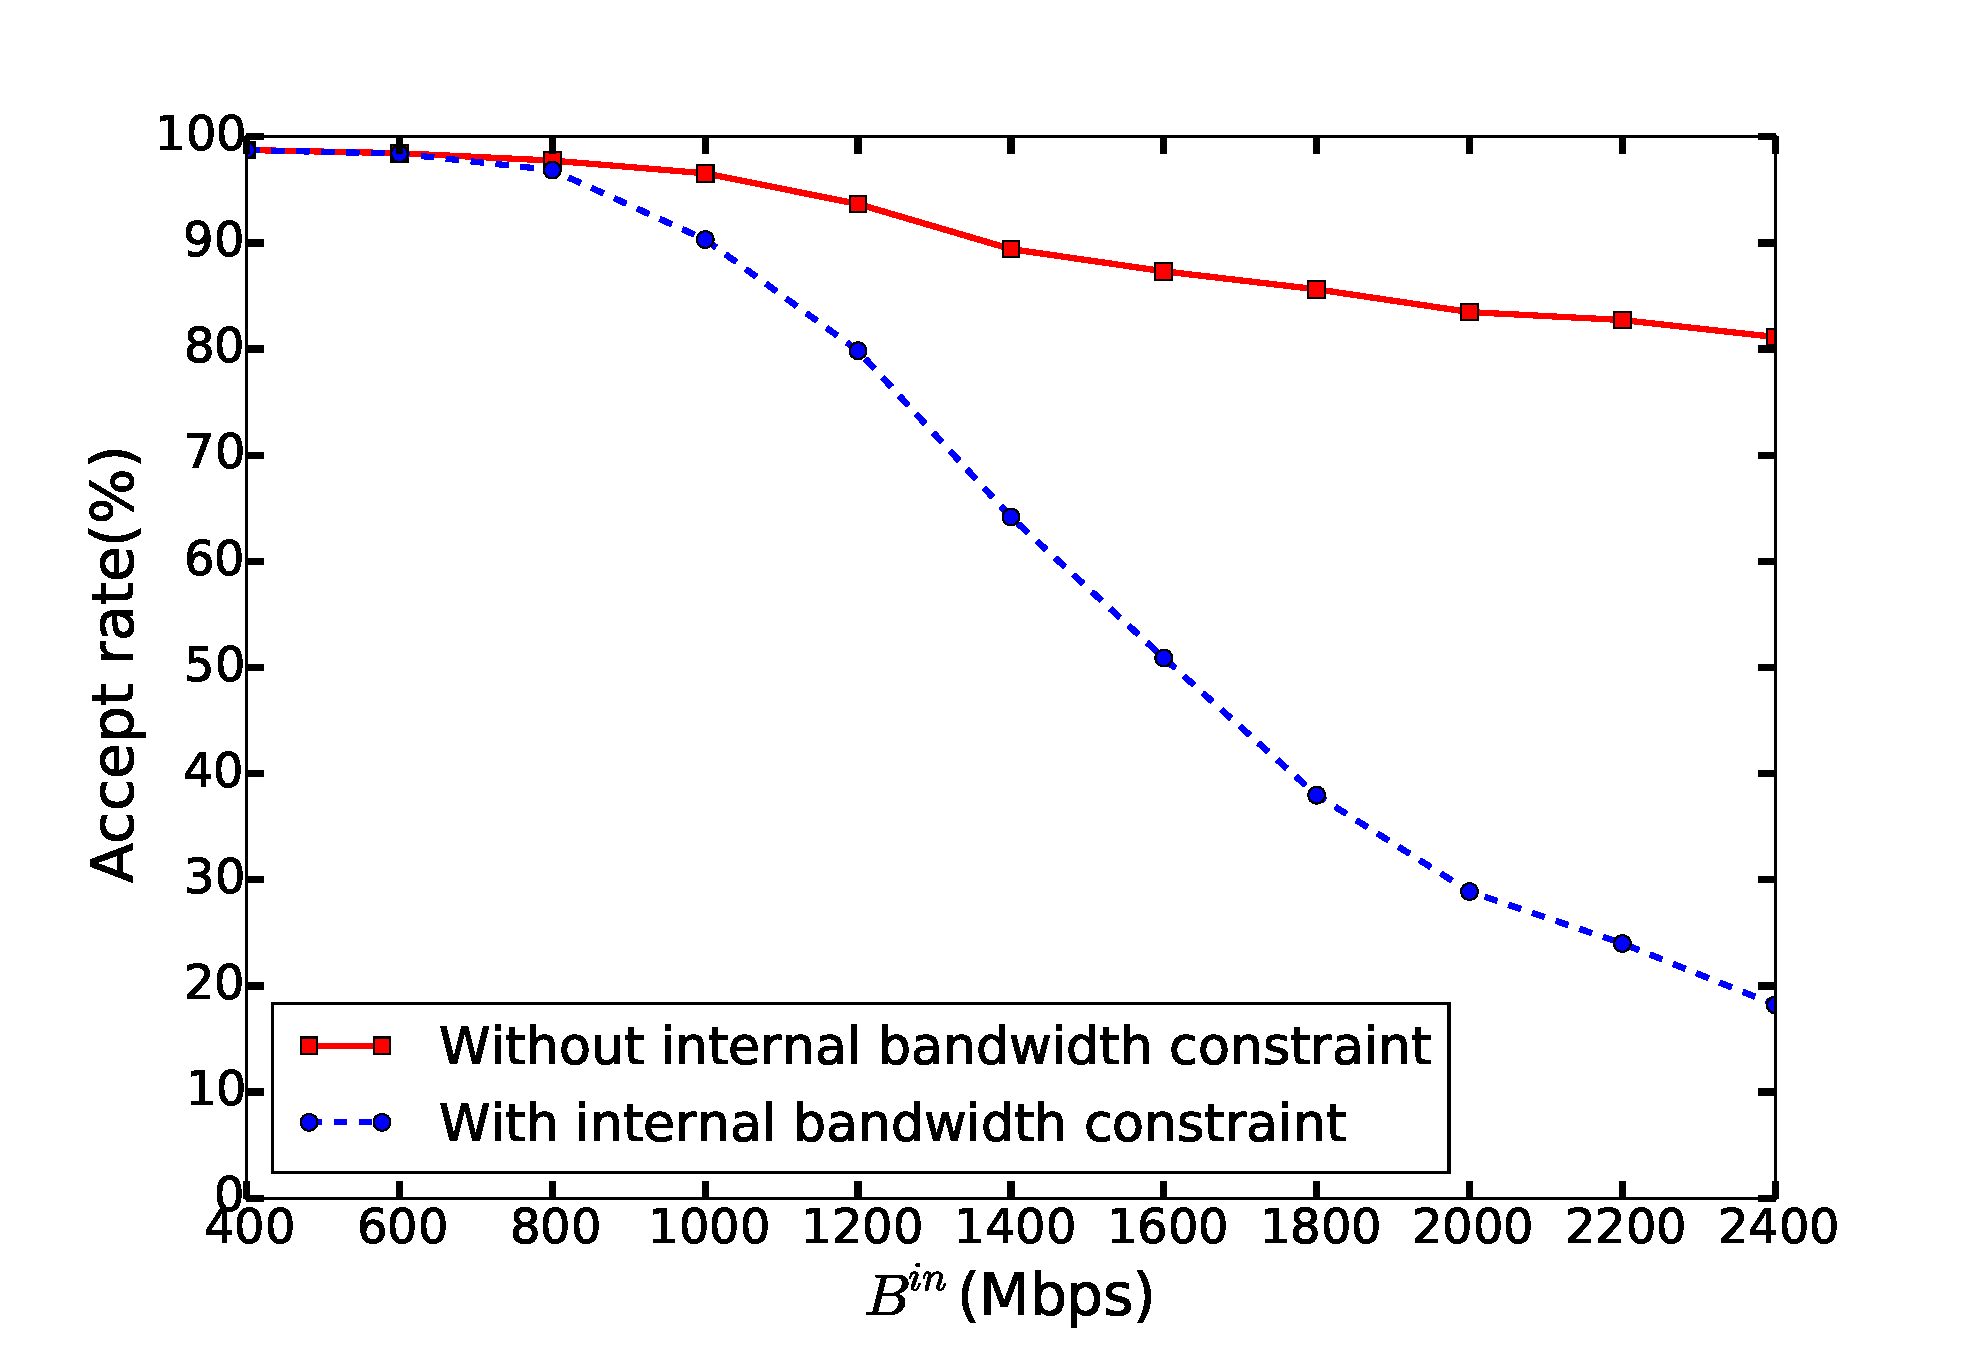
\includegraphics[width=3.2in,height=2.0in]{fig/pm_constraint.pdf}
	\caption{Accept rate with or without internal bandwidth constraint}
	\label{fig:pm_constraint}
\end{figure}
\end{comment}
\section{Evaluation}\label{sec:simulation}
We evaluate our placement algorithm via simulation. We build a tree-like three-layer network topology, which is inspired by a real cloud datacenter with 30000+ VMs. Each ToR switch is connected to 40 physical servers with 10Gbps NICs. And every PM is divided into 8 slots. The oversubscribtion ration are 4:1 at the leaf level and 10:1 at the spine layer.  

To simulate the tenant request, we model the intra-tenant bandwidth $B^{in}$ and inter-tenant bandwidth $B^{ex}$ to follow normal distribution. The maximal capacity $b_k$ of each type of middleboxes also follows the normal distribution with average value as 1000. For simplicity, we assume that each tenant request only contains one middlebox chain. The length of the middlebox chain is randomly selected in [1,3]. And the number of APP VMs required corresponding to a middlebox chain is equally distributed between 3 to 10. The fraction of open tenants is set to be 10\% while the fraction of client tenants is defined as 25\%. Furthermore, there are also some tenants that have communication request with each other. We set the fraction of these tenants to be 15\%.  

We consider two placement algorithms: 1) a VM placement strategy (without scaling requirement) described in Stratos \cite{stratos12} which logically partitions the VMs into per-rack partitions and places them with minimal inter-partition communication; 2) our placement algorithm(EMB) that places the MB and APP VMs carefully given in Algorithm 1. To compare the two placement algorithms, we create tenant requests continuously until the datacenter could not accept tenant request any more.

We first evaluate the tenant accept rates under different $B^{in}$ and $B^{ex}$ in Fig. \ref{fig:accept_rate}.
%Fig. \ref{fig:accept_rate_bin} shows 
In Fig. \ref{fig:accept_rate_bin}, we consider 
the accept rate of tenant requests with various intra-tenant communication demands ($B^{in}$). $B^{in}$=1200 means that the tenants’ $B^{in}$ follows the normal distribution with average value as 1200 and variation equal to $B^{in}$/3=400. In Fig. \ref{fig:accept_rate_bin}, we find that both algorithms have similar accept rates with varying $B^{in}$. 

The results of accept rate with varying external bandwidth ($B^{ex}$) are shown in Fig. \ref{fig:accept_rate_bex}. Similarly, $B^{ex}$=1200 means that $B^{ex}$ follows the normal distribution with average value of 1200 and variation as $B^{ex}$/3=400. Obviously, EMB can always accept tenant requests reposefully. And even with large $B^{ex}$, EMB can keep a relatively high accept rate. While the accept rate of Stratos drops quickly when $B^{ex}$ is greater than 800Mbps. This is because Stratos usually occupies more bandwidth resource in higher level links. More specifically, the number of total VMs required for tenant requests increases as $B^{ex}$ increases since we need more middlebox instances to process a larger external traffic. This leads to an increased demand for VM slots resource in the data center, and the tenant requests are forced to spread their VMs across more racks. The placement strategy used in Stratos is more likely to select the racks that reside across several subtrees to accommodate the tenant request, which may cause a big waste of bandwidth in the high-level links. While our placement algorithm always tries to select the lowest-level subtree that has sufficient VM slots for the tenant, which can save the precious bandwidth resource of the high level links effectively. Thus, EMB is helpful to allow the provider to accommodate more tenant requests while reducing the bandwidth utilization of high-level links which allows more future tenant requests to be accepted.

Fig. \ref{fig:vm_util} shows the VM slots utilization of the datacenter under different $B^{in}$ and $B^{ex}$. We can see that the results of VM slots utilization have similar changing trends compared to the accept rates shown in Fig. \ref{fig:accept_rate}.
%Fig. \ref{fig:accept_rate_bin} and Fig. \ref{fig:accept_rate_bex}. 
This is reasonable since higher accept rates represent that there are more requests accepted and more VM slots resources allocated.  

For a better understanding of above results, we then evaluate the downlink bandwidth utilization of core-aggregation and ToR-PM links. Note that the servers are on the same layer of the three-level network topology, if there is one download bandwidth consumption, there must be another upload bandwidth consumption correspondingly. This leads to the result that the download and upload results are similar to each other. Hence, we just show the results of the download bandwidth here. The results are shown in Fig. \ref{fig:bw_util}, where the x-coordinate shows the intra-tenant bandwidth ($B^{in}$) consumption, and the y-coordinate shows the average bandwidth utilization of the core-aggregation and ToR-PM download links in the two subfigures respectively. In Fig. \ref{fig:bw_util}(a), we can see that EMB has lower bandwidth utilization than Stratos in the core-aggregation links. On the other side, EMB has a higher utilization of the PM-ToR links shown in Fig. \ref{fig:bw_util}(b) which, in turn, proves the effect of lowest-level subtrees locality placement of our algorithm. To sum up, EMB can save the bandwidth efficiently of high-level links which are usually the bottlenecks for most oversubscription data center networks while making the best of low-level links’ bandwidth. 

%We then evaluate the impact of $B^{in}$ and bandwidth constraint inside a PM. The bandwidth constraint within a physical machine limits the number of VMs allowed to be placed. The experimental results are shown in Fig. \ref{fig:pm_constraint}. It is observable that when internal bandwidth constraint is considered, the accept rate of tenant requests quickly drops as $B^{in}$ increases. As the link capacity and internal constraint are the same in our simulation, a request is always limited by the internal PM constraint first, which reduces the number of available VM slots and leads to a lower accept rate.

\section{Conclusion}\label{sec:final}
Since middleboxes are widely used in current networks, it is essential to consider middleboxes when embedding predicable virtual networks. This paper tries to fill the gap. To achieve this goal, this paper first models the tenant's requirement of software middleboxes and applications. By augumenting software middleboxes as VMs in the Tenant Application Graph, an VMs placement algorithm, called EMB, is proposed to place these VMs (including both normal application VMs and virtual middleboxes) in the underlying infrastructure. The evaluation results have shown that the proposed virtual middleboxes placement algorithm can effectively use the resource of multi-tenant datacenters and provide performance guarantee for tenants.   

 


%Abstraction can truely reflect the characteristic of tenant requirement
%The abstraction can map to the physical environment to satisfy the requirement but reduce the consumption of resources. 


%\section*{Acknowledgment}
%The authors thank anonymous reviewers for the work and constructive comments and suggestions. 


\bibliographystyle{IEEEtran}
\bibliography{reference}

\appendix
To address the problem of unpredictable MB performance, instead of allocating new resources of VMs and network after MBs are placed in datacenters, we introduce a probability model to represent the variable resource requirement of individual tenant. Through statistically multiplexing on VMs, we are able to balance the physical resources consumption and scalability requirement of software MBs. 

%To deal with scalability issue of software middleboxes with minimum bandwidth guarantee, 
We re-examine the MBs request and take the time-varying resource requirements of MBs into consideration. Specifically, the MBs' requirement is composed of a basic requirement and a variable requirement with probablity. Based on this model, we replace the $\langle T, M \rangle$ in Section \ref{sec:modelformb} with tuples $\langle T, M, m, P\rangle$, where $T$ and $M$  denote the type of MBs and the corresponding number of VMs in the basic requirement, and $m$ denotes the number of VMs in the variable subrequirement with probability $P$. For example, given $T=\{\text{FW, IDS, LB}\}, M=\{ 2, 4, 2\}, m=\{1, 2, 1\}, P=\{0.3, 0.2, 0.3\}$, we then know that the tenant request for 2 firewall MBs and the request may increase to $2+1=3$ MBs with probability of 0.2. Similarly, 4 IDS MBs (resp. 2 LB MBs) are needed with probability 0.8 (resp. 0.7) and 6 IDS MBs (resp. 3 LB MBs) with a probability of 0.2 (resp. 0.3). In summary, a tenant's request can be specified by multiple virtual networks (VNs) and each VN can be specified by an eight-tuple $<N, B^{in}, B^{ex}, dependencies, T, M, m, P>$. It allows elasticity by having a probability model for the number of MBs needed in each VN. 

If multiple units of subrequirement do not occur simultaneously, we can provide few redundancy to tradeoff between utilization and availability. By sharing free VMs between variable subrequirements, a specific MB can be soon deployed on the free VM once the scale up/out requirement comes. Although the subrequirement occurs with a probability less than 1, the collision may happen if there is not enough VM provided. To guarantee the performance, we apply the probabilistic model to solve this problem. For simplicity, we reuse the notation $M$ to indicate how many types of MBs are required by tenant. Let $X_{i}$ indicate whether the $i$-th subrequirement occurs. Assuming the resource requirement of different middleboxes are independent, the probability of the collision happening on one supplement VM is
\begin{align}
&Pr\left[ \sum_{i=1}^{M} X_{i} > 1 \right] & \nonumber \\
&= 1-\prod_{i=1}^{M}(1-p_{i})-\sum_{i=1}^{M}\left(p_{i}\prod_{k\in[1,M], k\neq i}(1-p_{k})\right)&
\end{align}
By providing enough number of free VMs during virtual middleboxes network deployment, the probability of collision can be guaranteed less than a collision threshold $\rho$ when the system is on board. The number of subrequirement $v$ can be determined by solving the following function:
\begin{equation}\label{equ:collision}  
		Pr\left[ \sum_{i=1}^{M} X_{i} \leq v \right] \leq \rho
\end{equation}
The collision probability $Pr\left[ \sum_{i=1}^{M} X_{i} \leq v \right]$ can be achieved based on the including excluding principle. Therefore, the total number of MB VMs to be allocated for one tenant is $|M|+v$, where $|M|$ is the number of basic MBs requirement and $v$ is the additional free VMs to be allocated as backup resources. Therefore, 

\begin{figure}
	\centering
		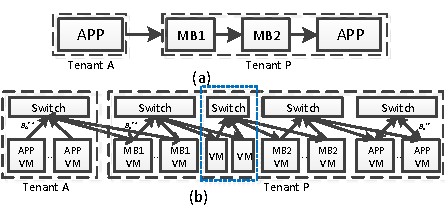
\includegraphics[width=3.3 in]{fig/scalability.pdf}
	\caption{Virtual Network Model. (a) the communication between two tenants; (b) cascade of TAG}
	\label{fig:scalability}
\end{figure}

Fig. \ref{fig:scalability} (B) uses the cascade of TAG model to abstract the communication dependency of VNs given in Fig. \ref{fig:scalability} (A). In comparison with Fig. \ref{fig:abstraction}, the VMs inside the blue dotted line are pre-allocated VMs for middleboxes subrequirement, which are shared by both types of middleboxes requests. If there are scale-out or failover request, specified MBs will be placed on these VMs to provide performance guarantee. If a tenant requires for multiple types of MBs, we can place free slots between cascade two types of MBs according to the expectation of their scalability. 

% that's all folks
\end{document}


